\documentclass{beamer}

\usepackage[utf8]{inputenc}
\usepackage{subfig}
\renewcommand{\thesubfigure}{\arabic{subfigure}}
\usepackage{ngerman}
\usetheme{focus}

% Captions
\usepackage{caption}
\captionsetup[figure]{labelformat=empty}

% Bibliography
\usepackage[citestyle=numeric,style=numeric,backend=biber]{biblatex}
\addbibresource{bibliography.bib}

\title{Prozedurale Generierung\\ von Wirbeltierskeletten}
\author{Nina Zimbel}
\institute{KIT -- Institut für Visualisierung und Datenanalyse}
\date{7.\ Juli 2020}

% Shorcuts
\newcommand{\zb}{z.\,B.\ }
\newcommand{\dash}{d.\,h.\ }
\newcommand{\va}{v.\,a.\ }
\newcommand{\ua}{u.\,a.\ }
\newcommand{\bzw}{bzw.\ }
\newcommand{\etc}{etc.\ }

\begin{document}

\begin{frame}
 \maketitle
\end{frame}

%-------------------
%\section{Einleitung}
%-------------------
\begin{frame}[plain]
 \centering
 \begin{figure}
  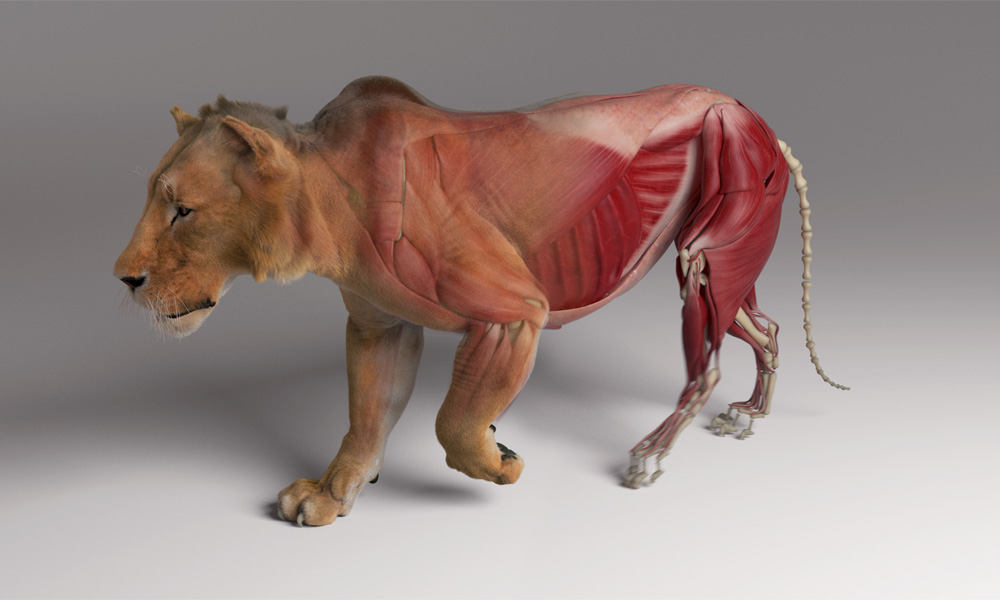
\includegraphics[width=\textwidth]{graphics/ziva-post2.jpg}
 \end{figure}
 \uncover<2>{\small Maya Plugin Ziva, wirklichkeitsgetreues Modell eines Löwen \cite{Ziva_Lion}}
\end{frame}

\begin{frame}[plain]
 \begin{figure}
  \centering
  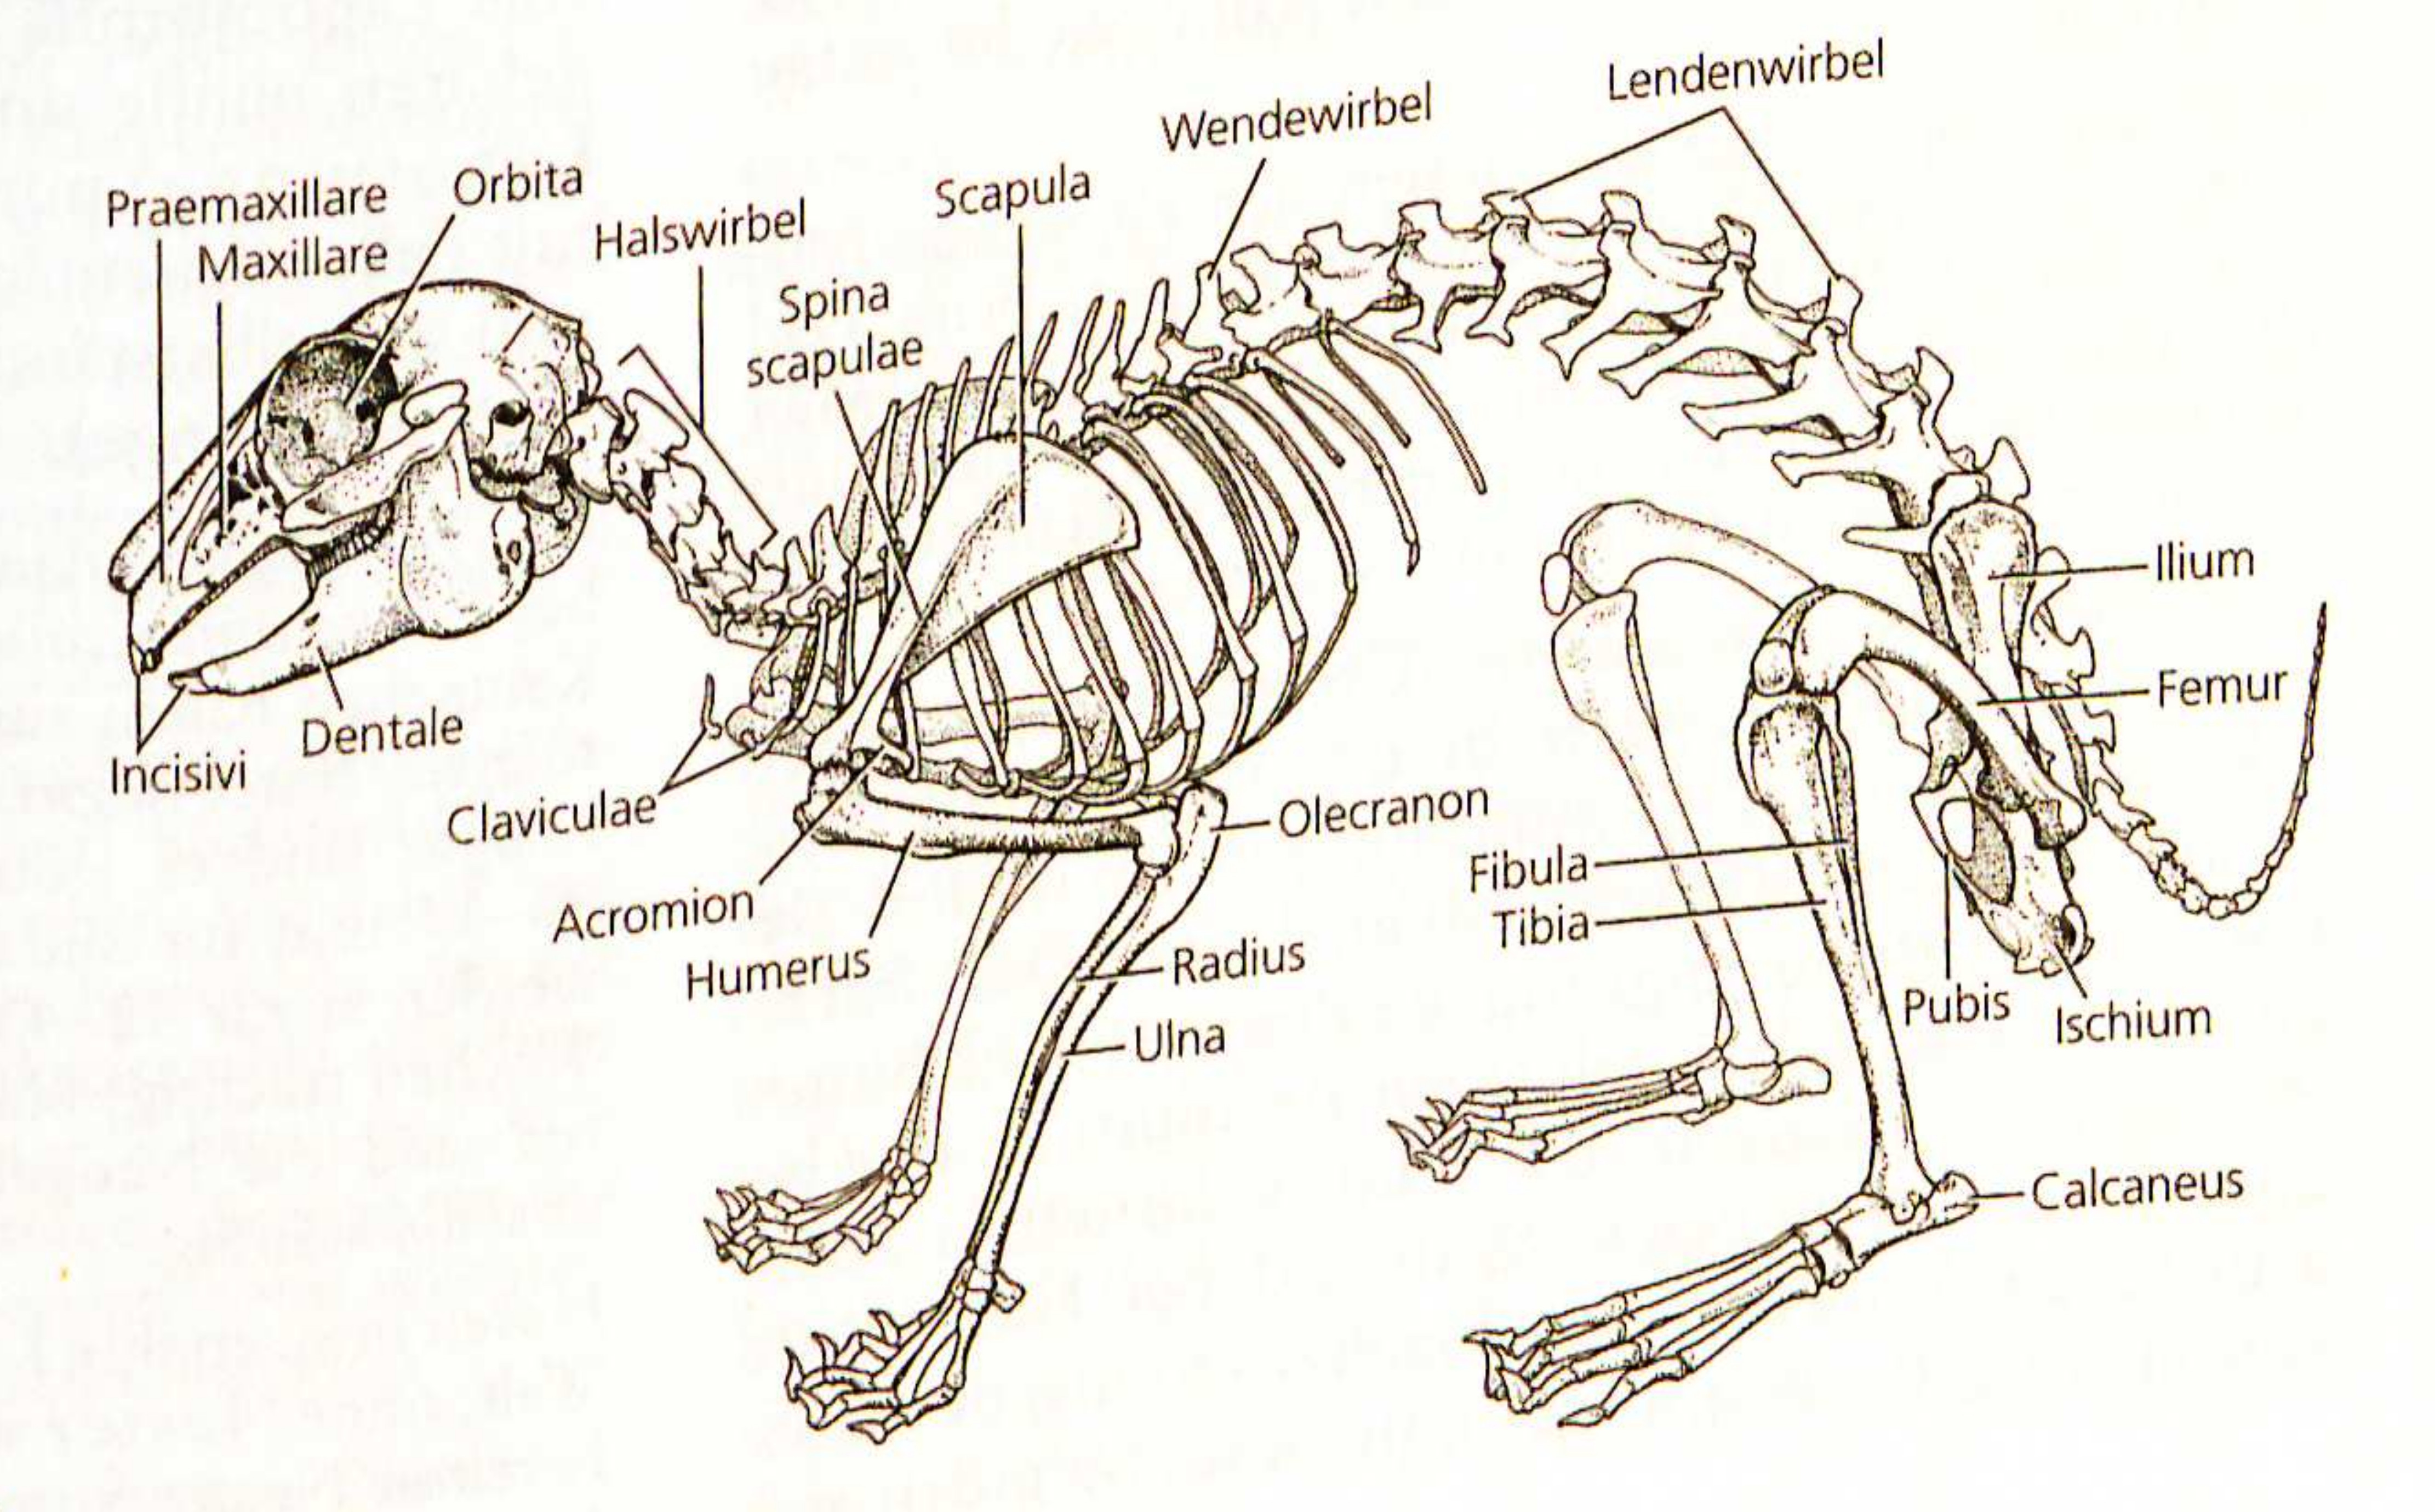
\includegraphics[width=\textwidth]{graphics/kaninchen.jpg}
  \caption{Skelett eines Kaninchens \cite{Spezielle_Zoologie}}
 \end{figure}
\end{frame}

\begin{frame}{Abstrahierter Grundbauplan}
 \begin{figure}
  \centering
  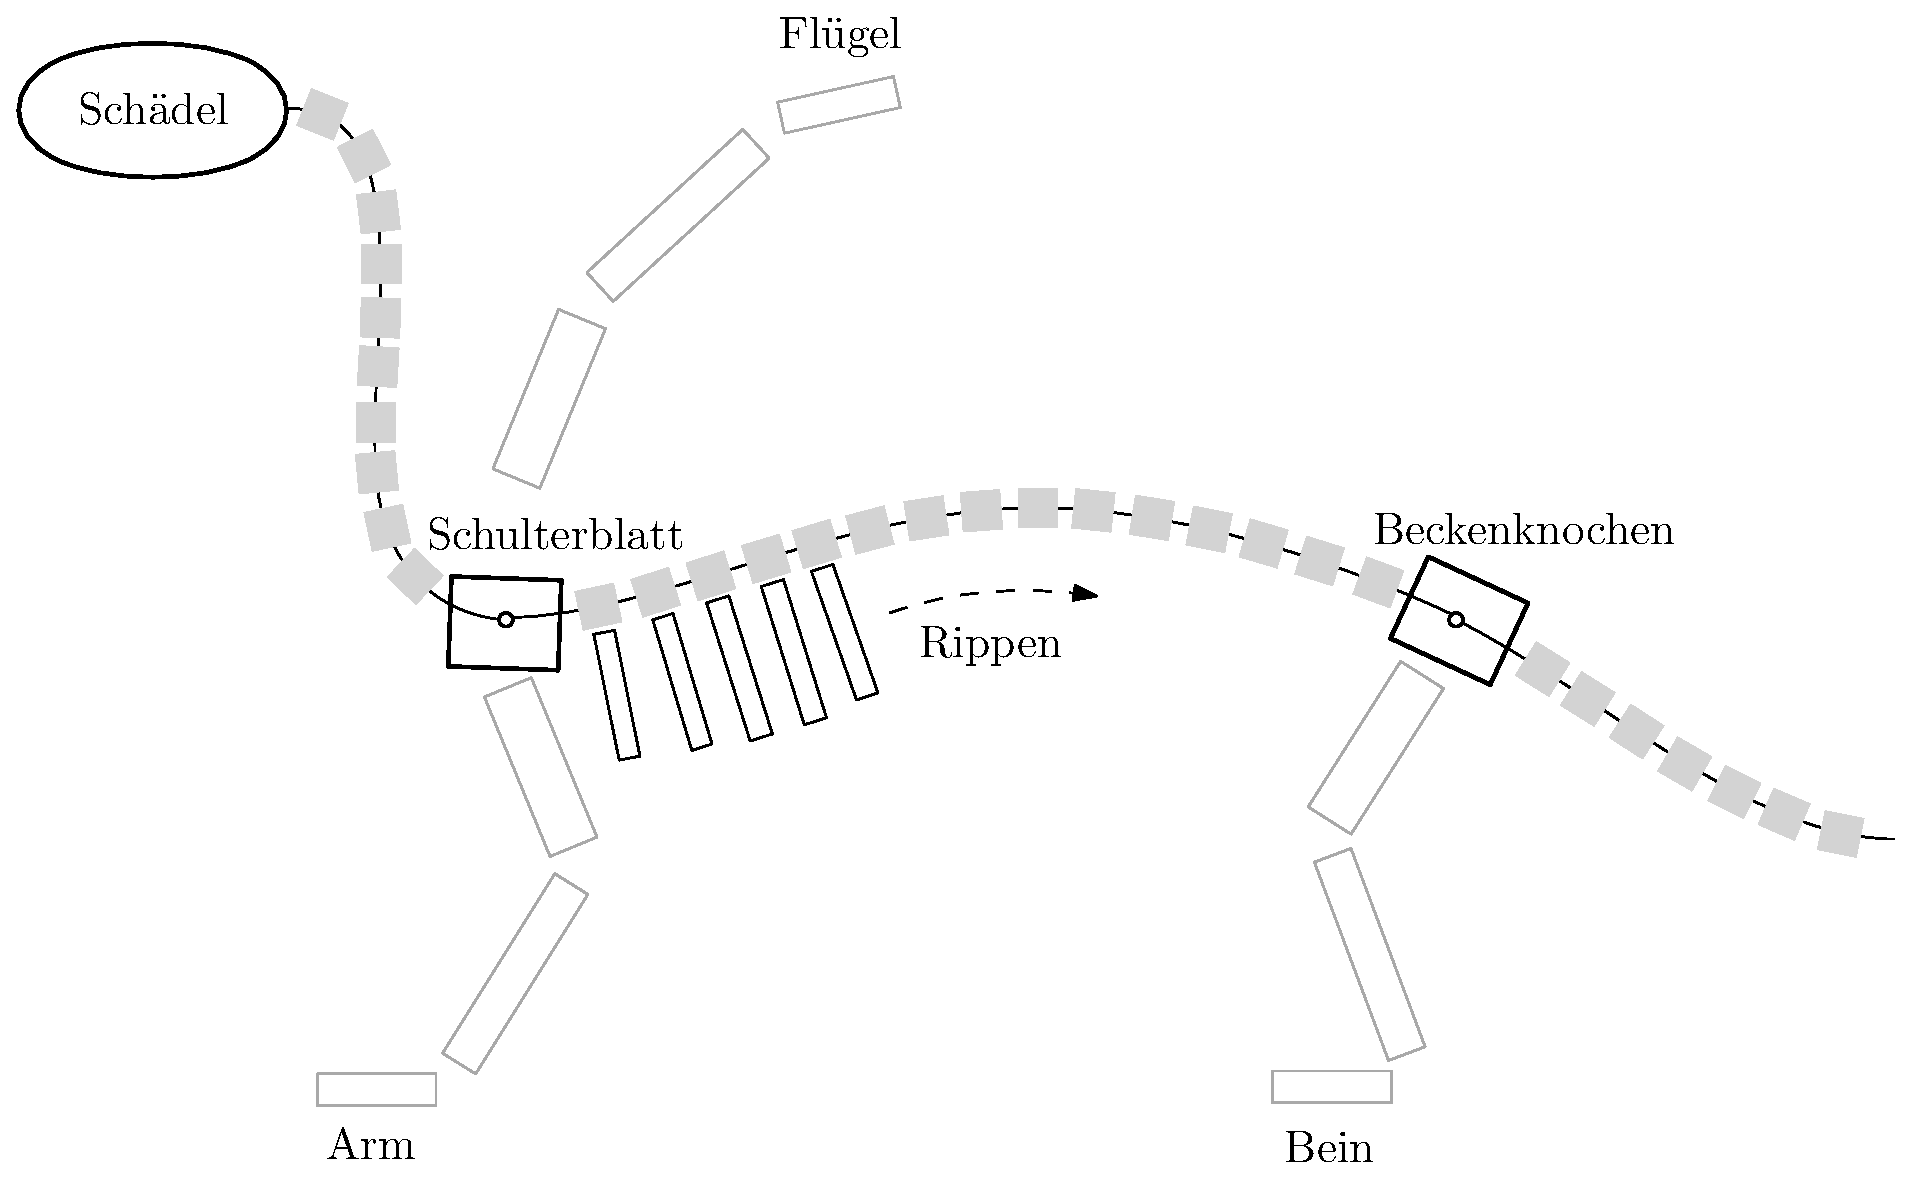
\includegraphics[width=\textwidth]{../graphics/skeletonPlan}
  %\caption{Abstrahierter Grundbauplan eines Wirbeltierskeletts}
 \end{figure}
\end{frame}

\begin{frame}{Gliederung}
 \begin{figure} 
  \subfloat[PCA]{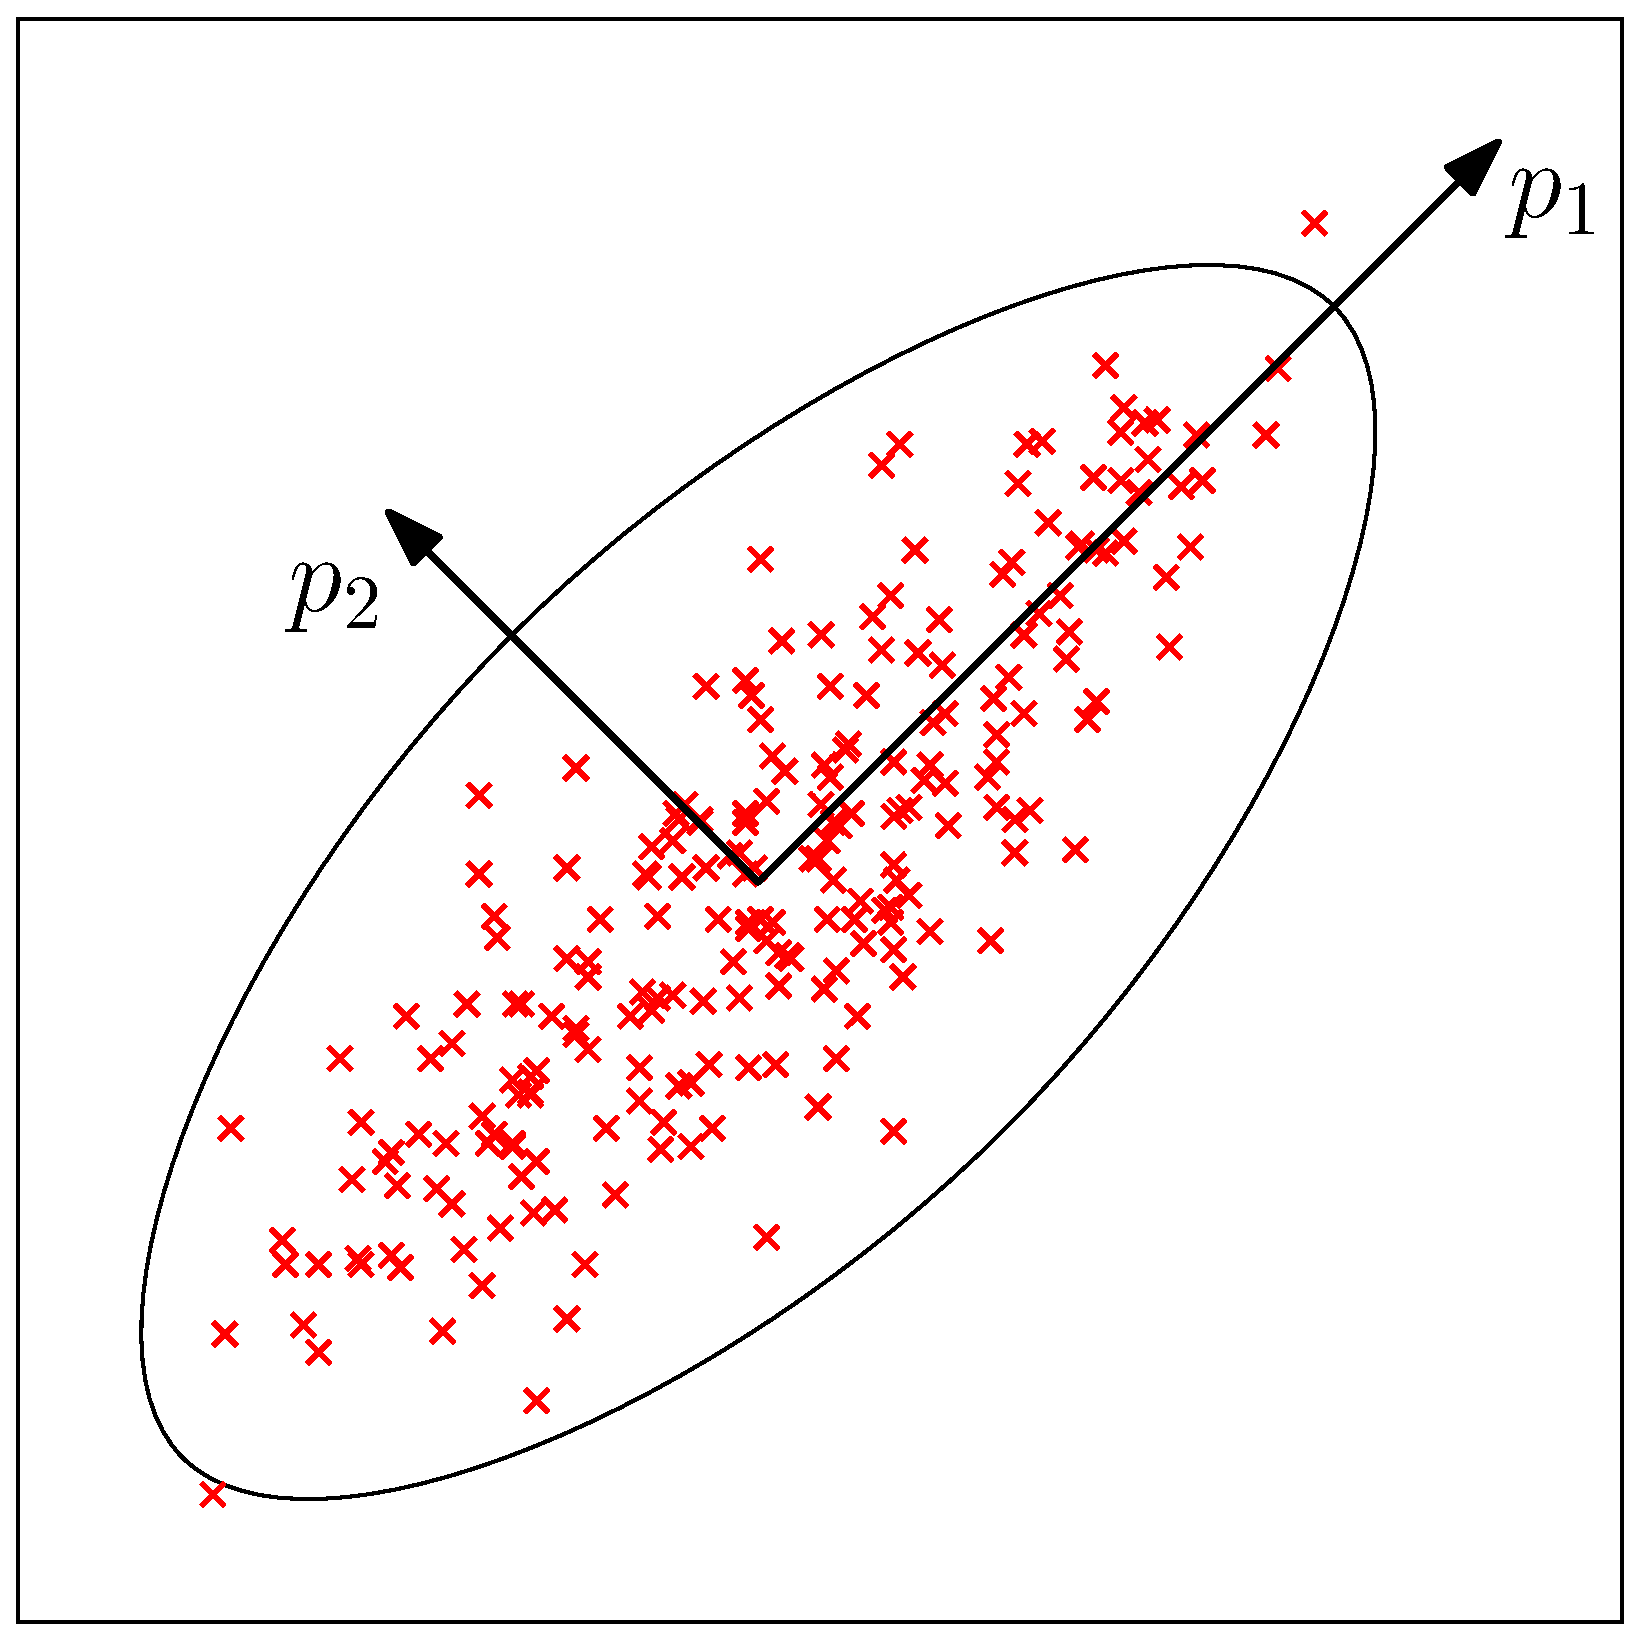
\includegraphics[height=0.4\textheight]{graphics/pca_without_global_coords}}~
  \subfloat[Ergebnisse]{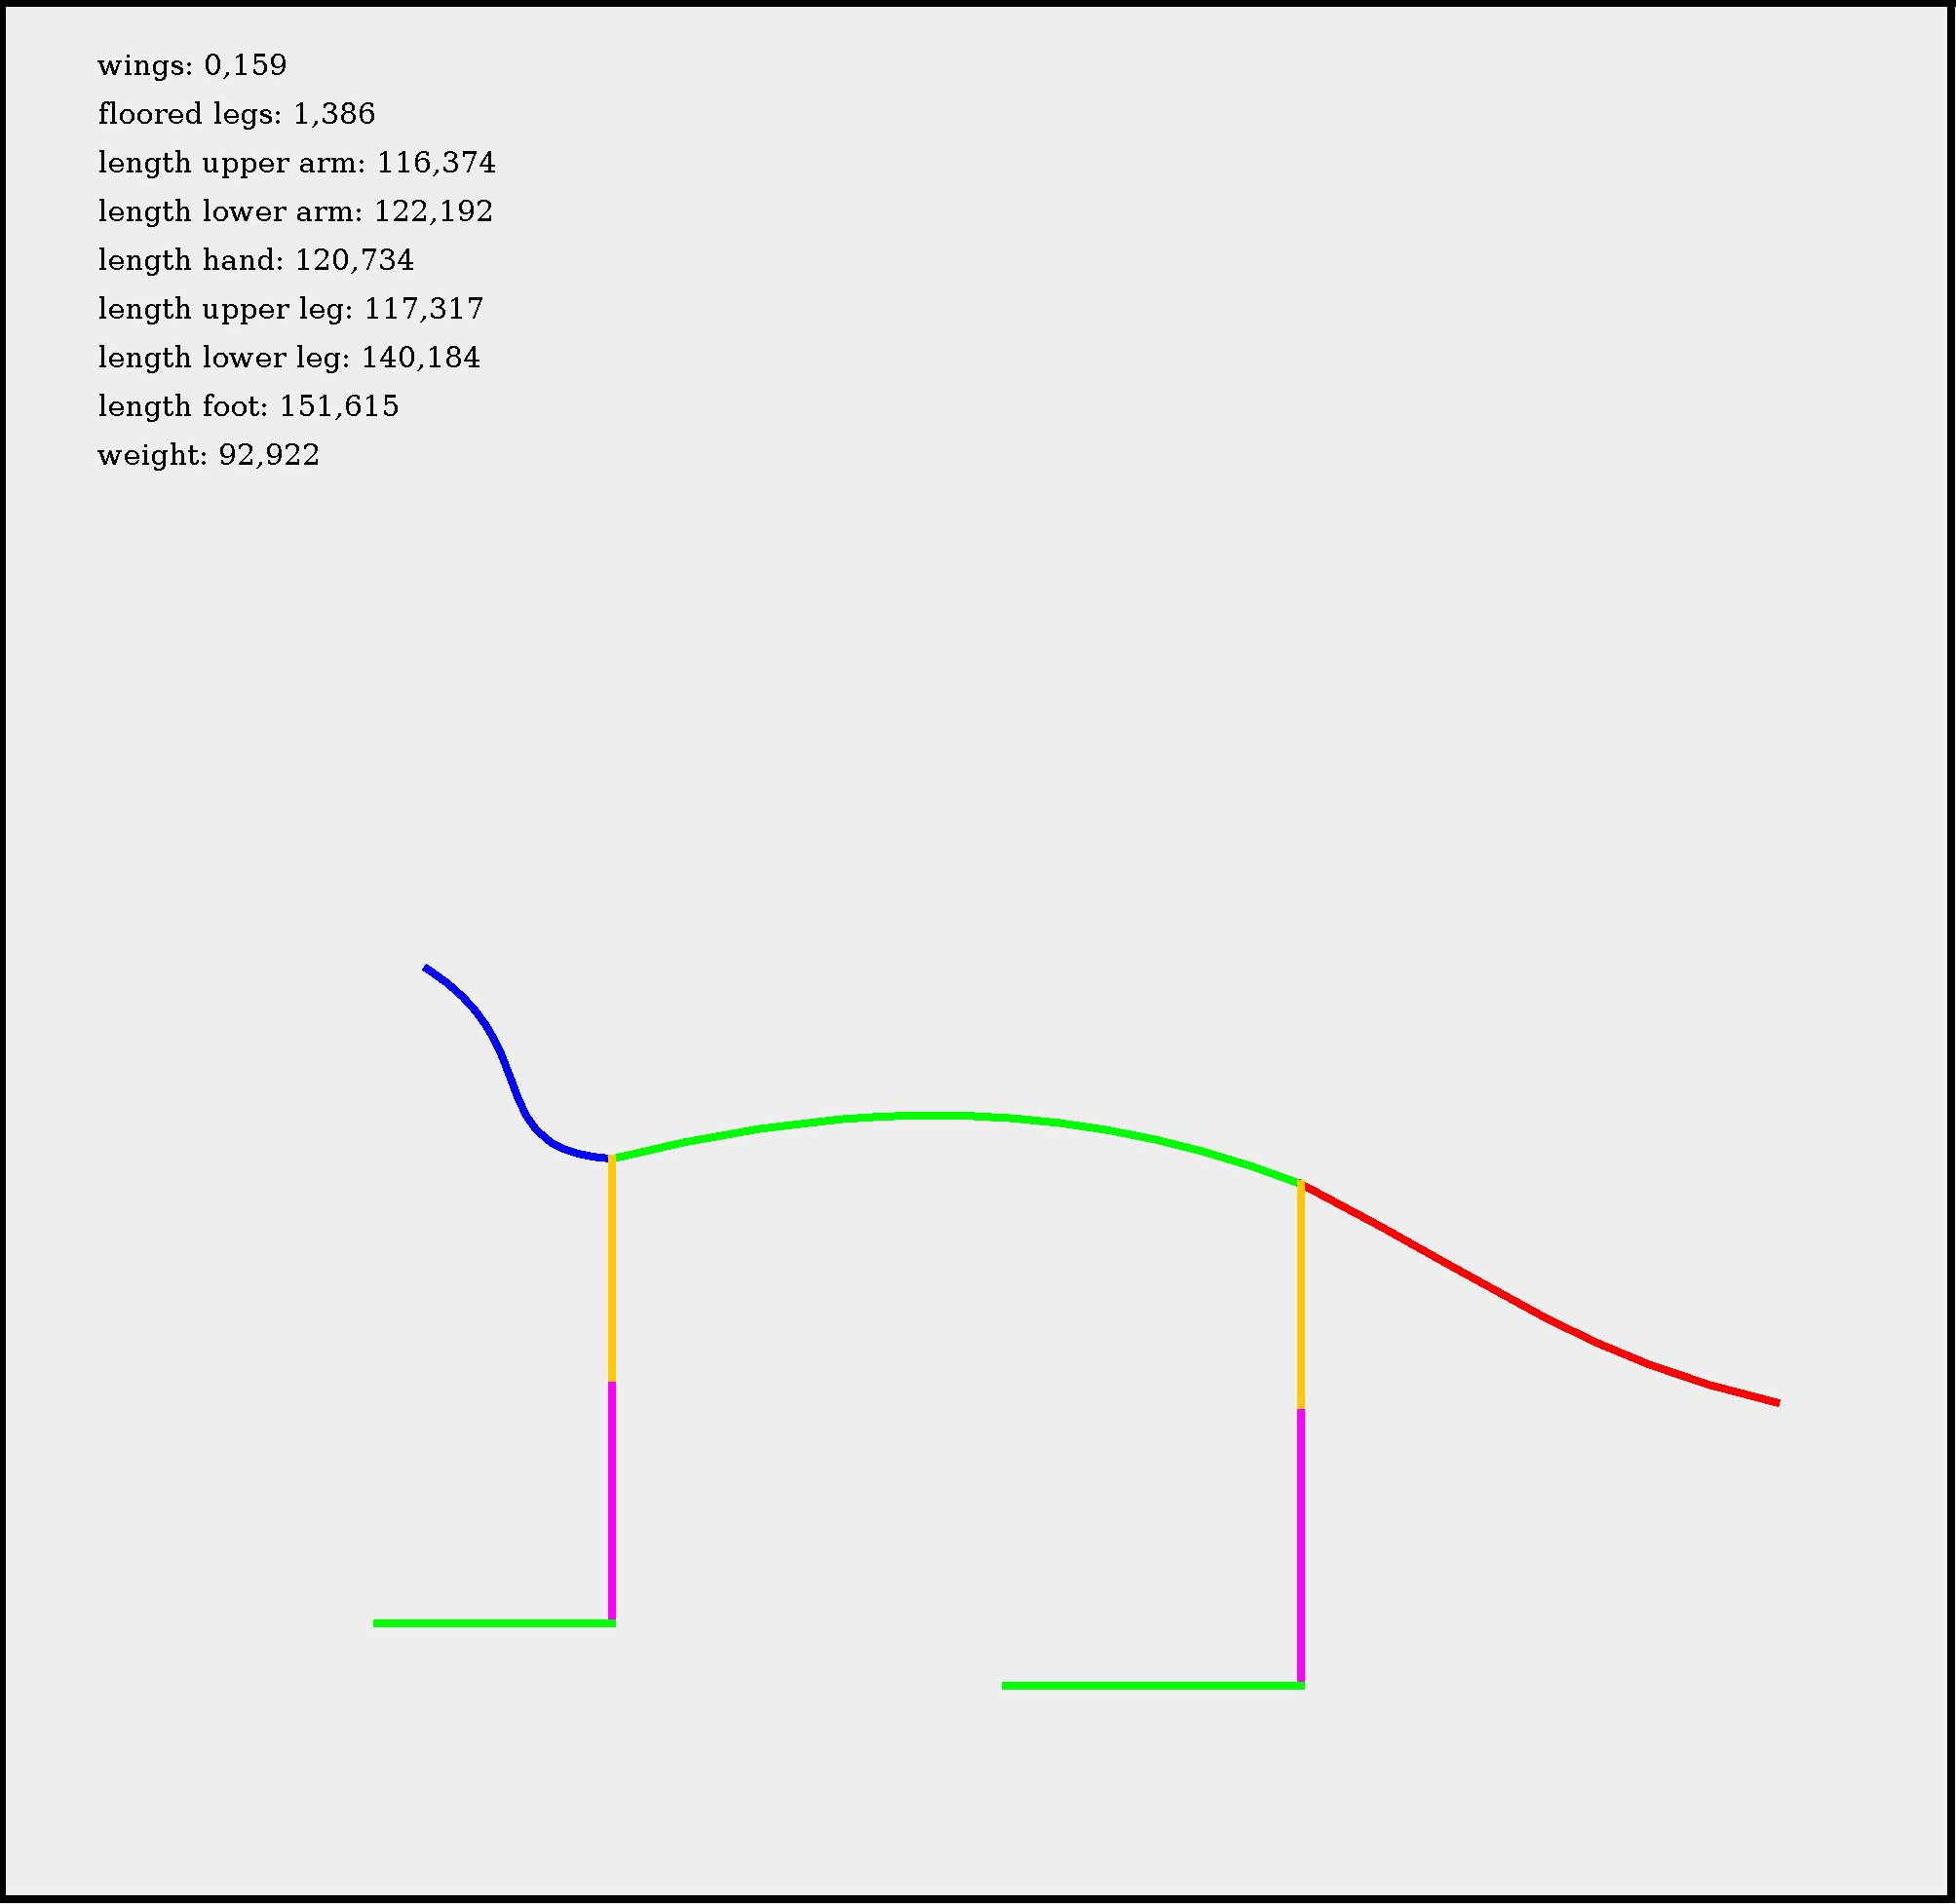
\includegraphics[height=0.4\textheight]{../../PCA/mean_log_weight_downscaled_wings_legs_and_weight(onlyBox,stroke4).jpg}}~
  \subfloat[Algorithmus]{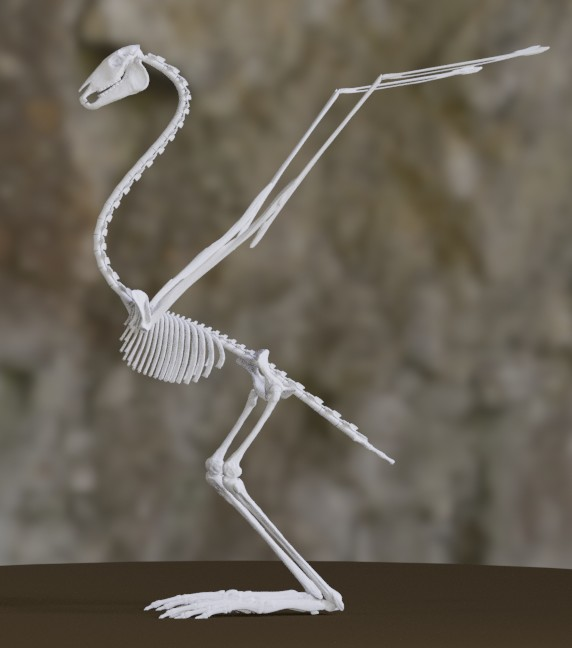
\includegraphics[height=0.4\textheight]{../../java_skeleton_generation/example_skeletons/bird.jpg}}~
%   \subfloat{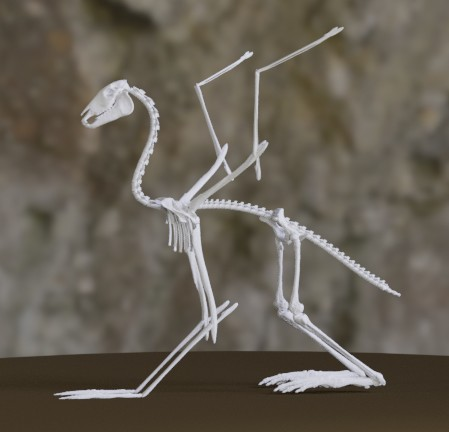
\includegraphics[height=0.4\textheight]{../../java_skeleton_generation/example_skeletons/pegasus.jpg}}
 \end{figure}
 \vfill
 \scriptsize Als Hintergrund wurde bei allen erzeugten Skeletten \cite{background} verwendet. Die Quellen der verwendeten externen 3D-Modelle sind in der Ausarbeitung zu finden.
\end{frame}


%-------------------------------------
\section{Principal Component Analysis}
%-------------------------------------
\begin{frame}{PCA}
 \begin{minipage}{0.6\textwidth}
   \begin{itemize}
    \item Gegeben: Menge normalverteilter $n$-dimensionaler Punkte
    \item Gesucht: Achsen des Hyperellipsoids $\rightarrow$ Basis des \emph{Konfigurationsraums}, der durch diese Achsen aufgespannt wird
  \end{itemize}
 \end{minipage}~
 \begin{minipage}{0.4\textwidth}
  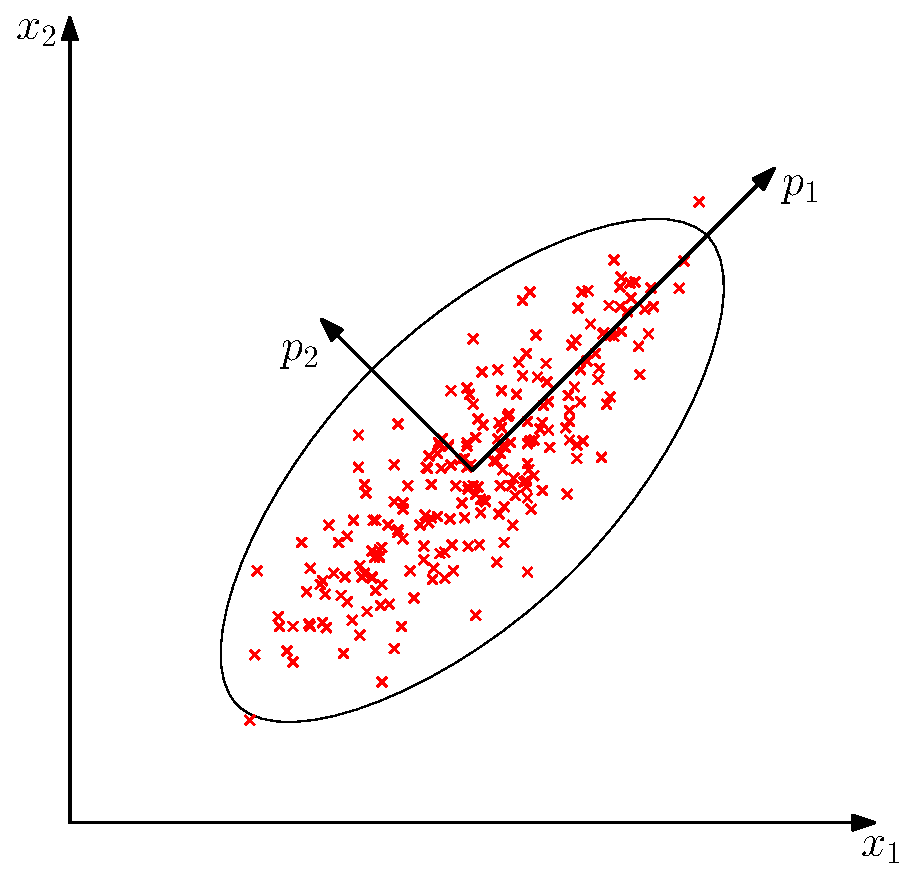
\includegraphics[width=\textwidth]{graphics/pca}
 \end{minipage}
 
 \uncover<2>{
  \begin{itemize}
   \item Verteilungen entlang der Achsen sind unabhängig voneinander $\rightarrow$ Erzeugung zufälliger Punkte mit gleicher Verteilung wie Eingabe möglich
  \end{itemize}
 }
\end{frame}

\begin{frame}{Warum PCA?}
 \begin{figure}
  \centering
  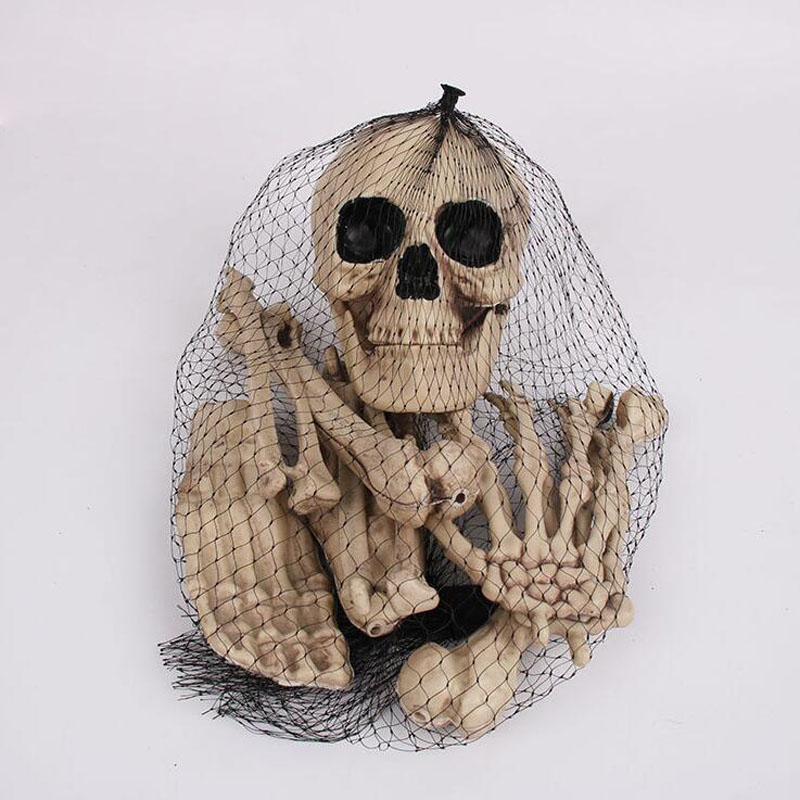
\includegraphics[height=0.7\textheight]{graphics/skeleton_set.jpg}
  \caption{\cite{skeleton_set}}
 \end{figure}
\end{frame}

\begin{frame}{Datenerhebung}
 \begin{minipage}{0.5\textwidth}
  \begin{itemize}
   \item 2D-Skelettbilder, \va aus Zoologiebüchern
   \item Merkmale: 
   \begin{itemize}
    \item Verlauf der Wirbelsäule (Bézierkurven)
    \item<2-> Länge der Knochen der Extremitäten
    \item<3-> Anzahl der Flügel
    \item<3-> Anzahl der Beine mit Bodenkontakt
    \item<4-> Gewicht
   \end{itemize}
  \end{itemize}
 \end{minipage}~
 \begin{minipage}{0.5\textwidth}
  \captionsetup{justification=centering}
  \begin{figure}
  \centering
  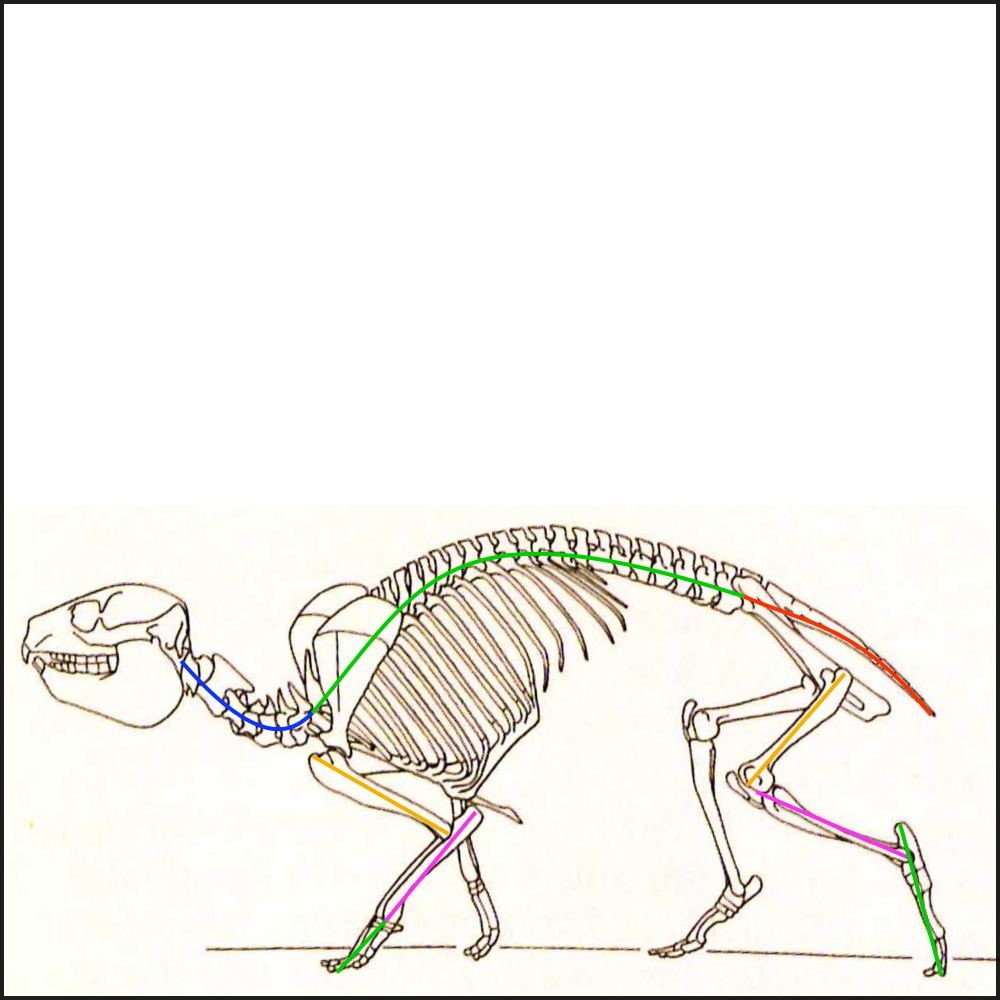
\includegraphics[width=\textwidth]{../../PCA/Skelettbilder/Klippschliefer_farbig.png}
  \caption{Annotiertes Skelett eines Klippschliefers \cite{Spezielle_Zoologie}}
 \end{figure}
 \end{minipage}
\end{frame}

\begin{frame}{Mittelwert}
 \captionsetup{justification=centering}
 \begin{figure}
  \centering
  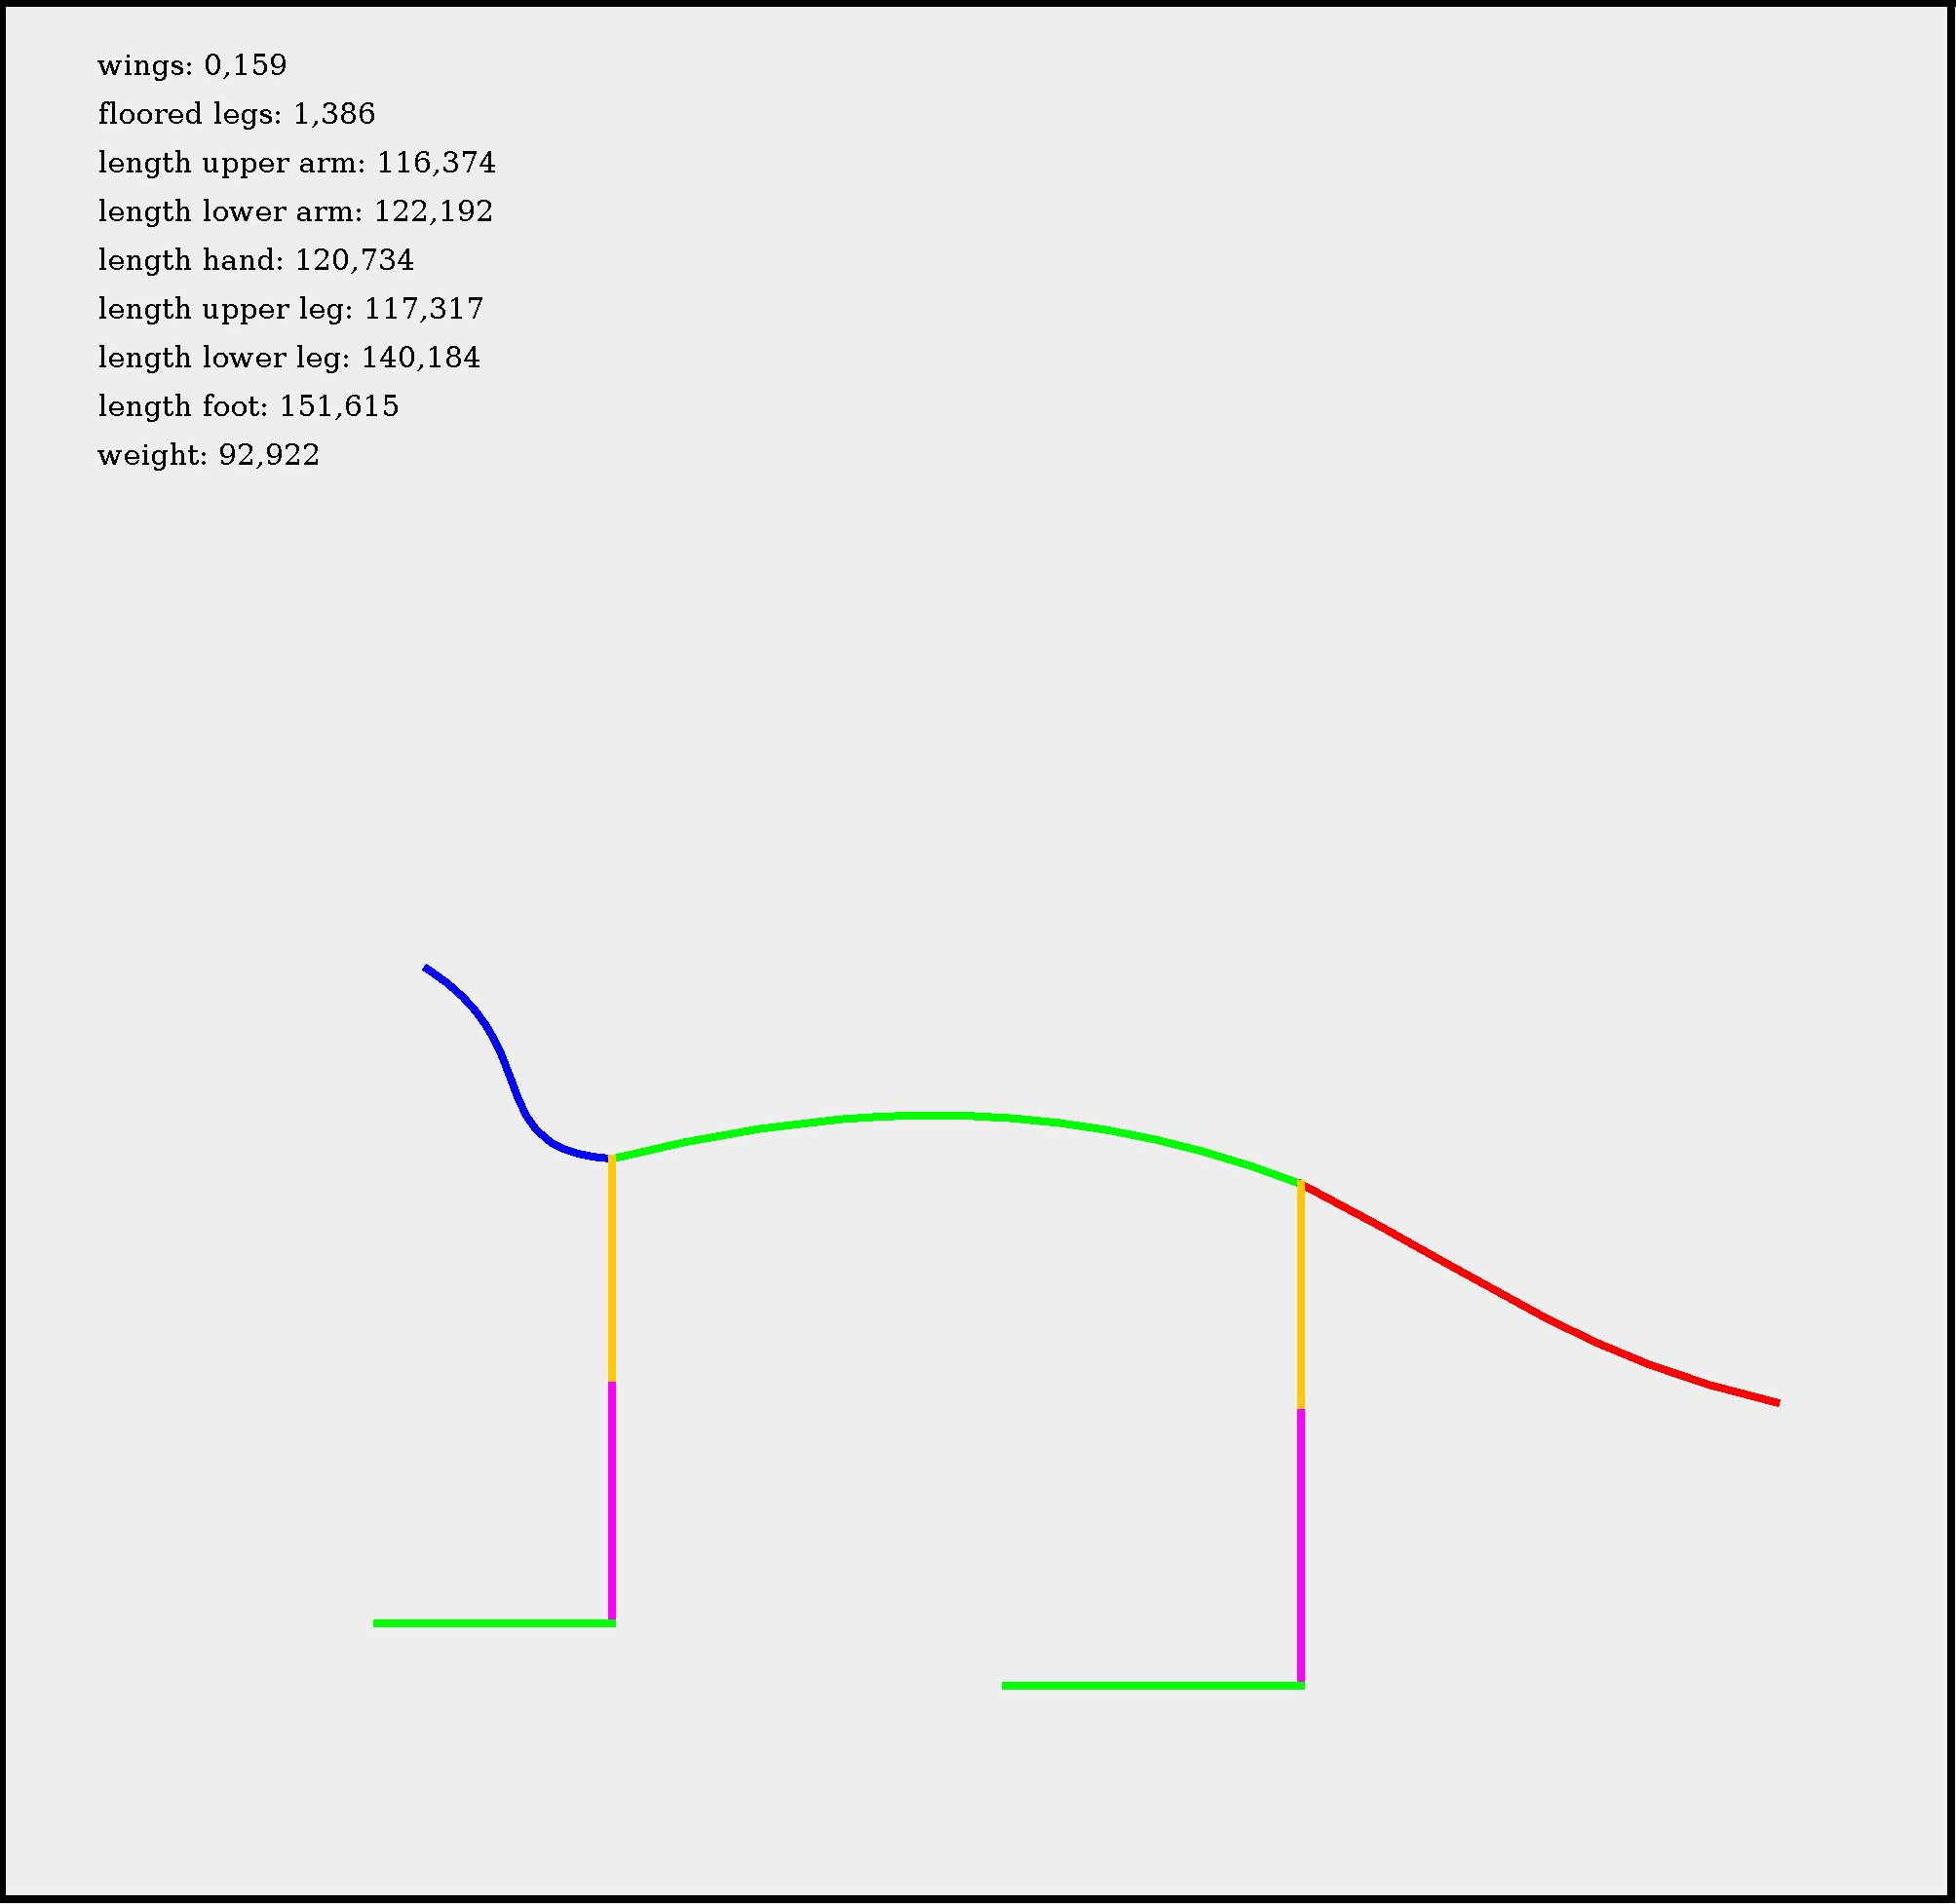
\includegraphics[height=0.6\textheight]{../../PCA/mean_log_weight_downscaled_wings_legs_and_weight(onlyBox,stroke4).jpg}
  \caption{Mittelwert der Eingabedaten\\ Flügelpaare $0{,}159$, Beinepaare mit Bodenkontakt $1{,}39$, Gewicht $93$kg}
 \end{figure}
\end{frame}

\begin{frame}{"`Bedeutung"' der Achsen}
 \begin{figure}
  \centering
  \subfloat{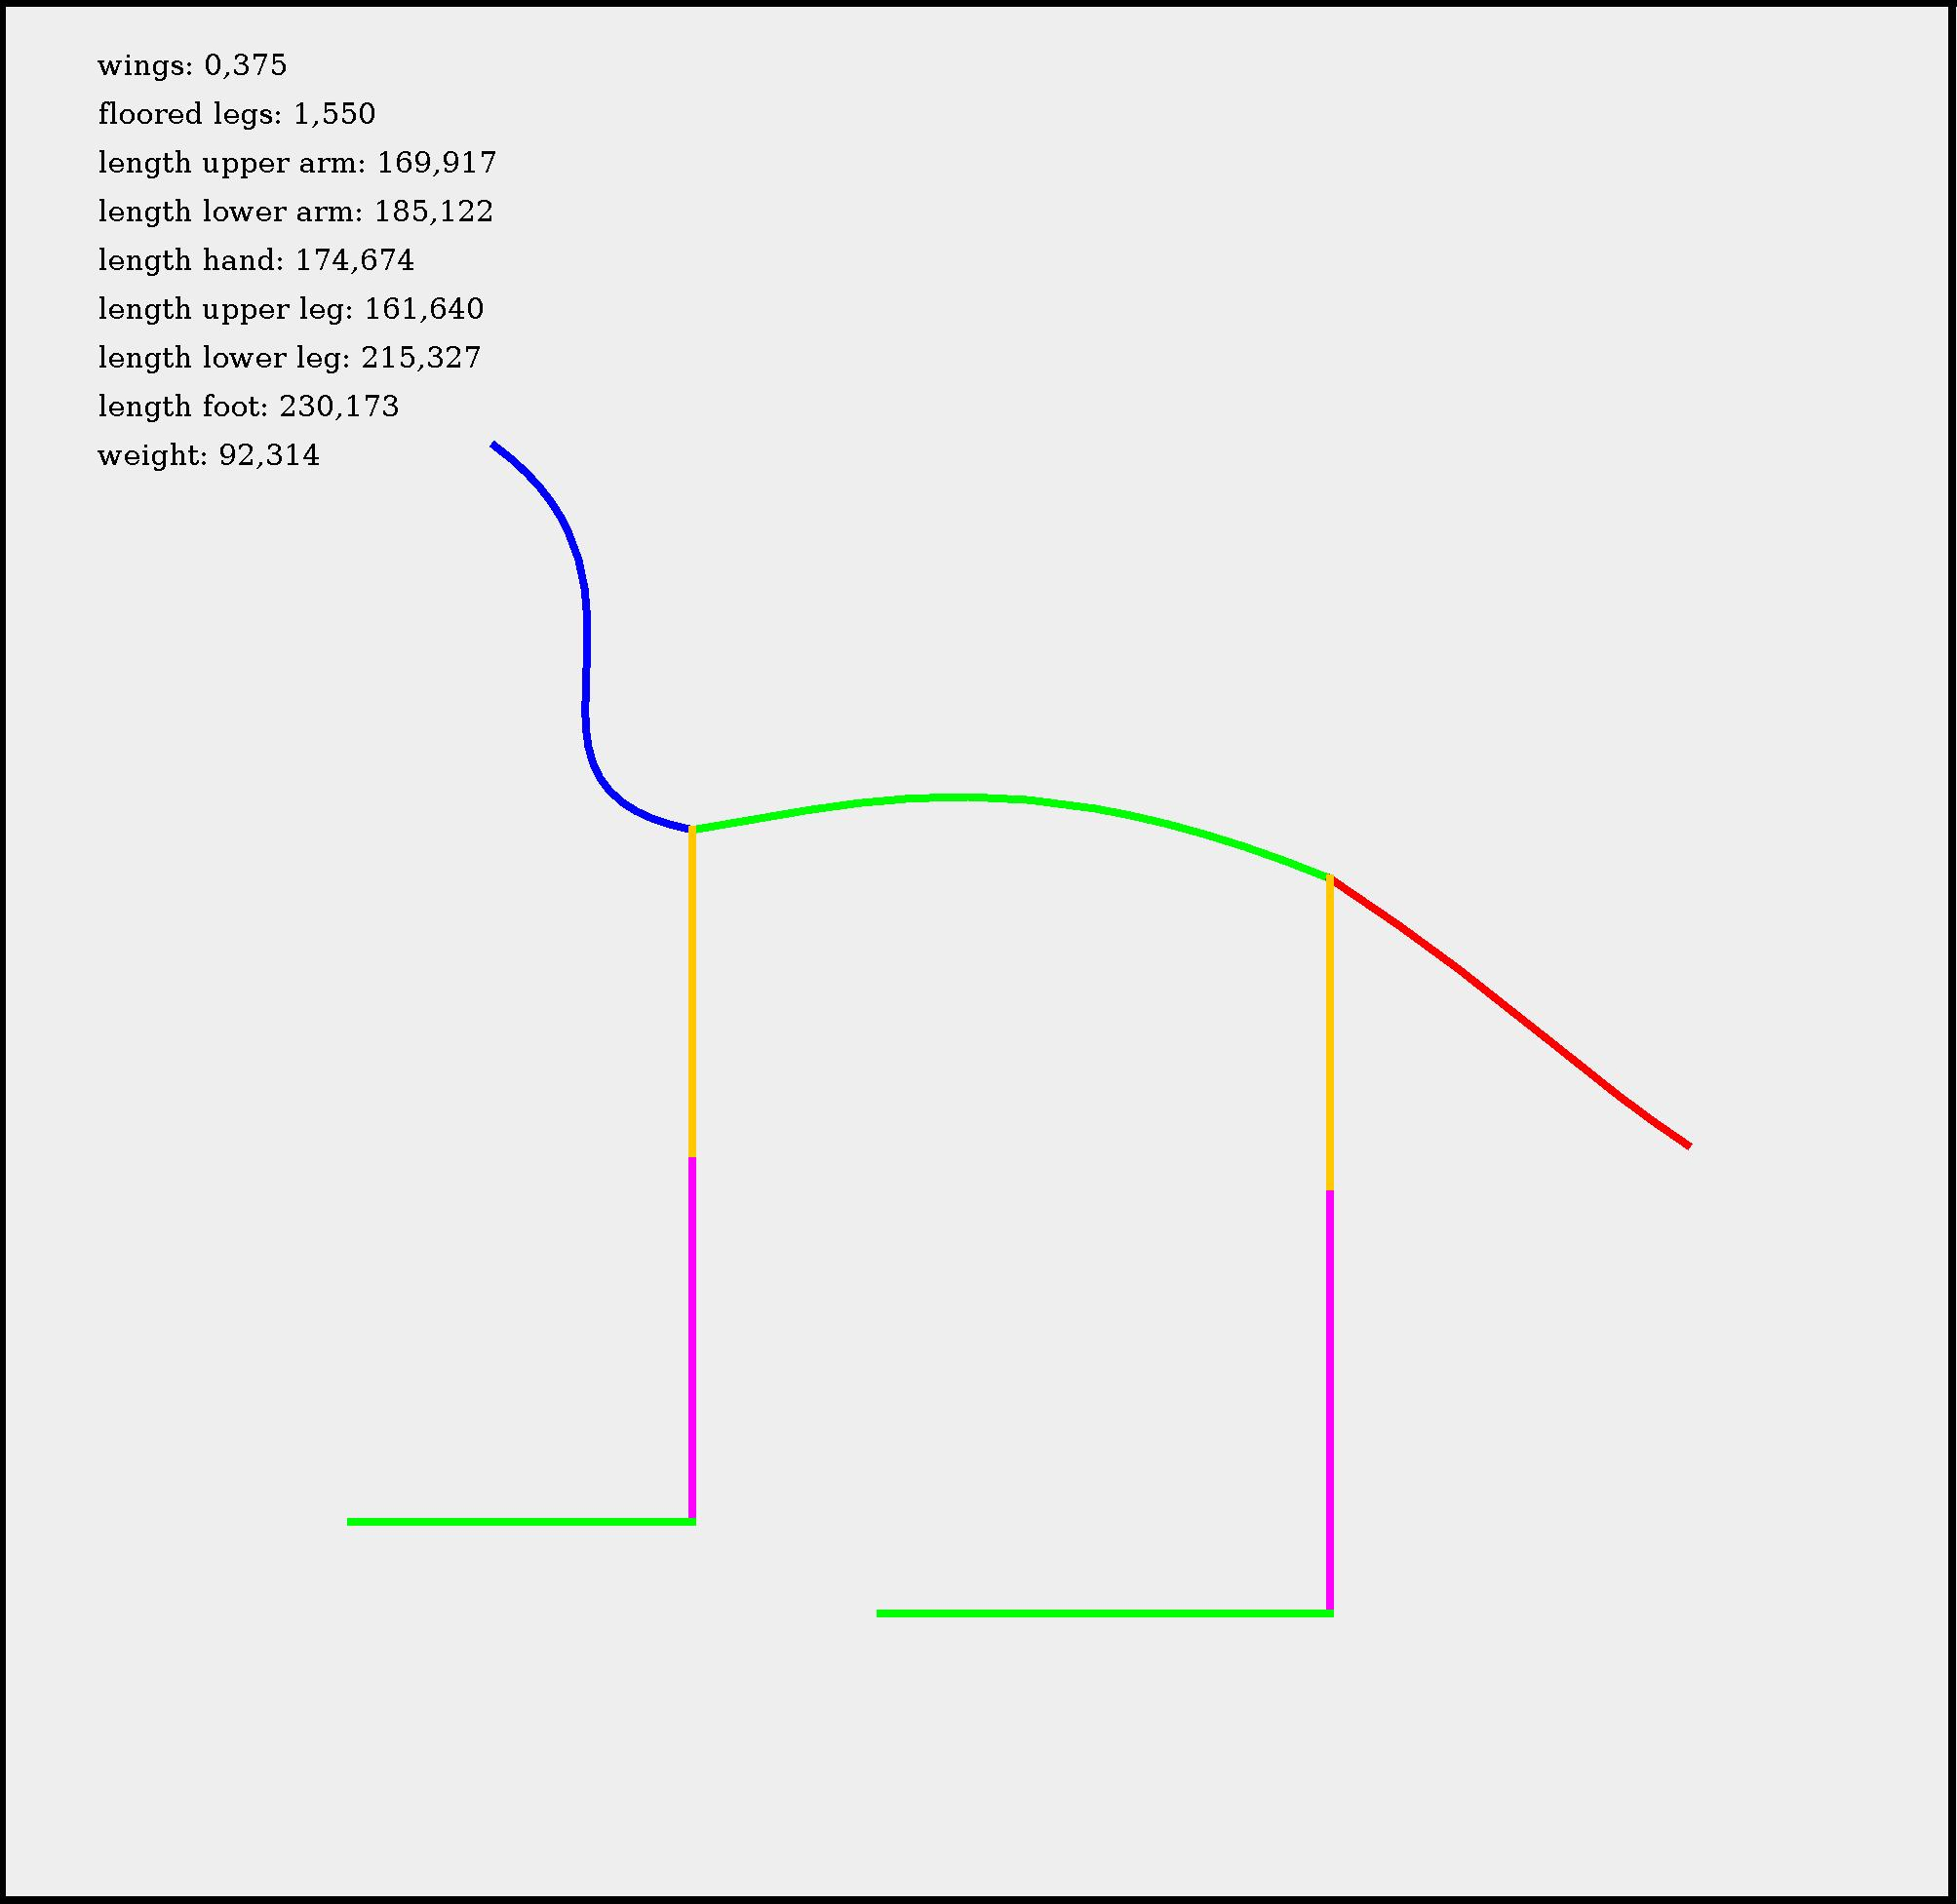
\includegraphics[height=0.5\textheight]{../../PCA/sqrtEV_log_weight_downscaled_wings_legs_and_weight/EV1_neg.jpg}}~
  \subfloat{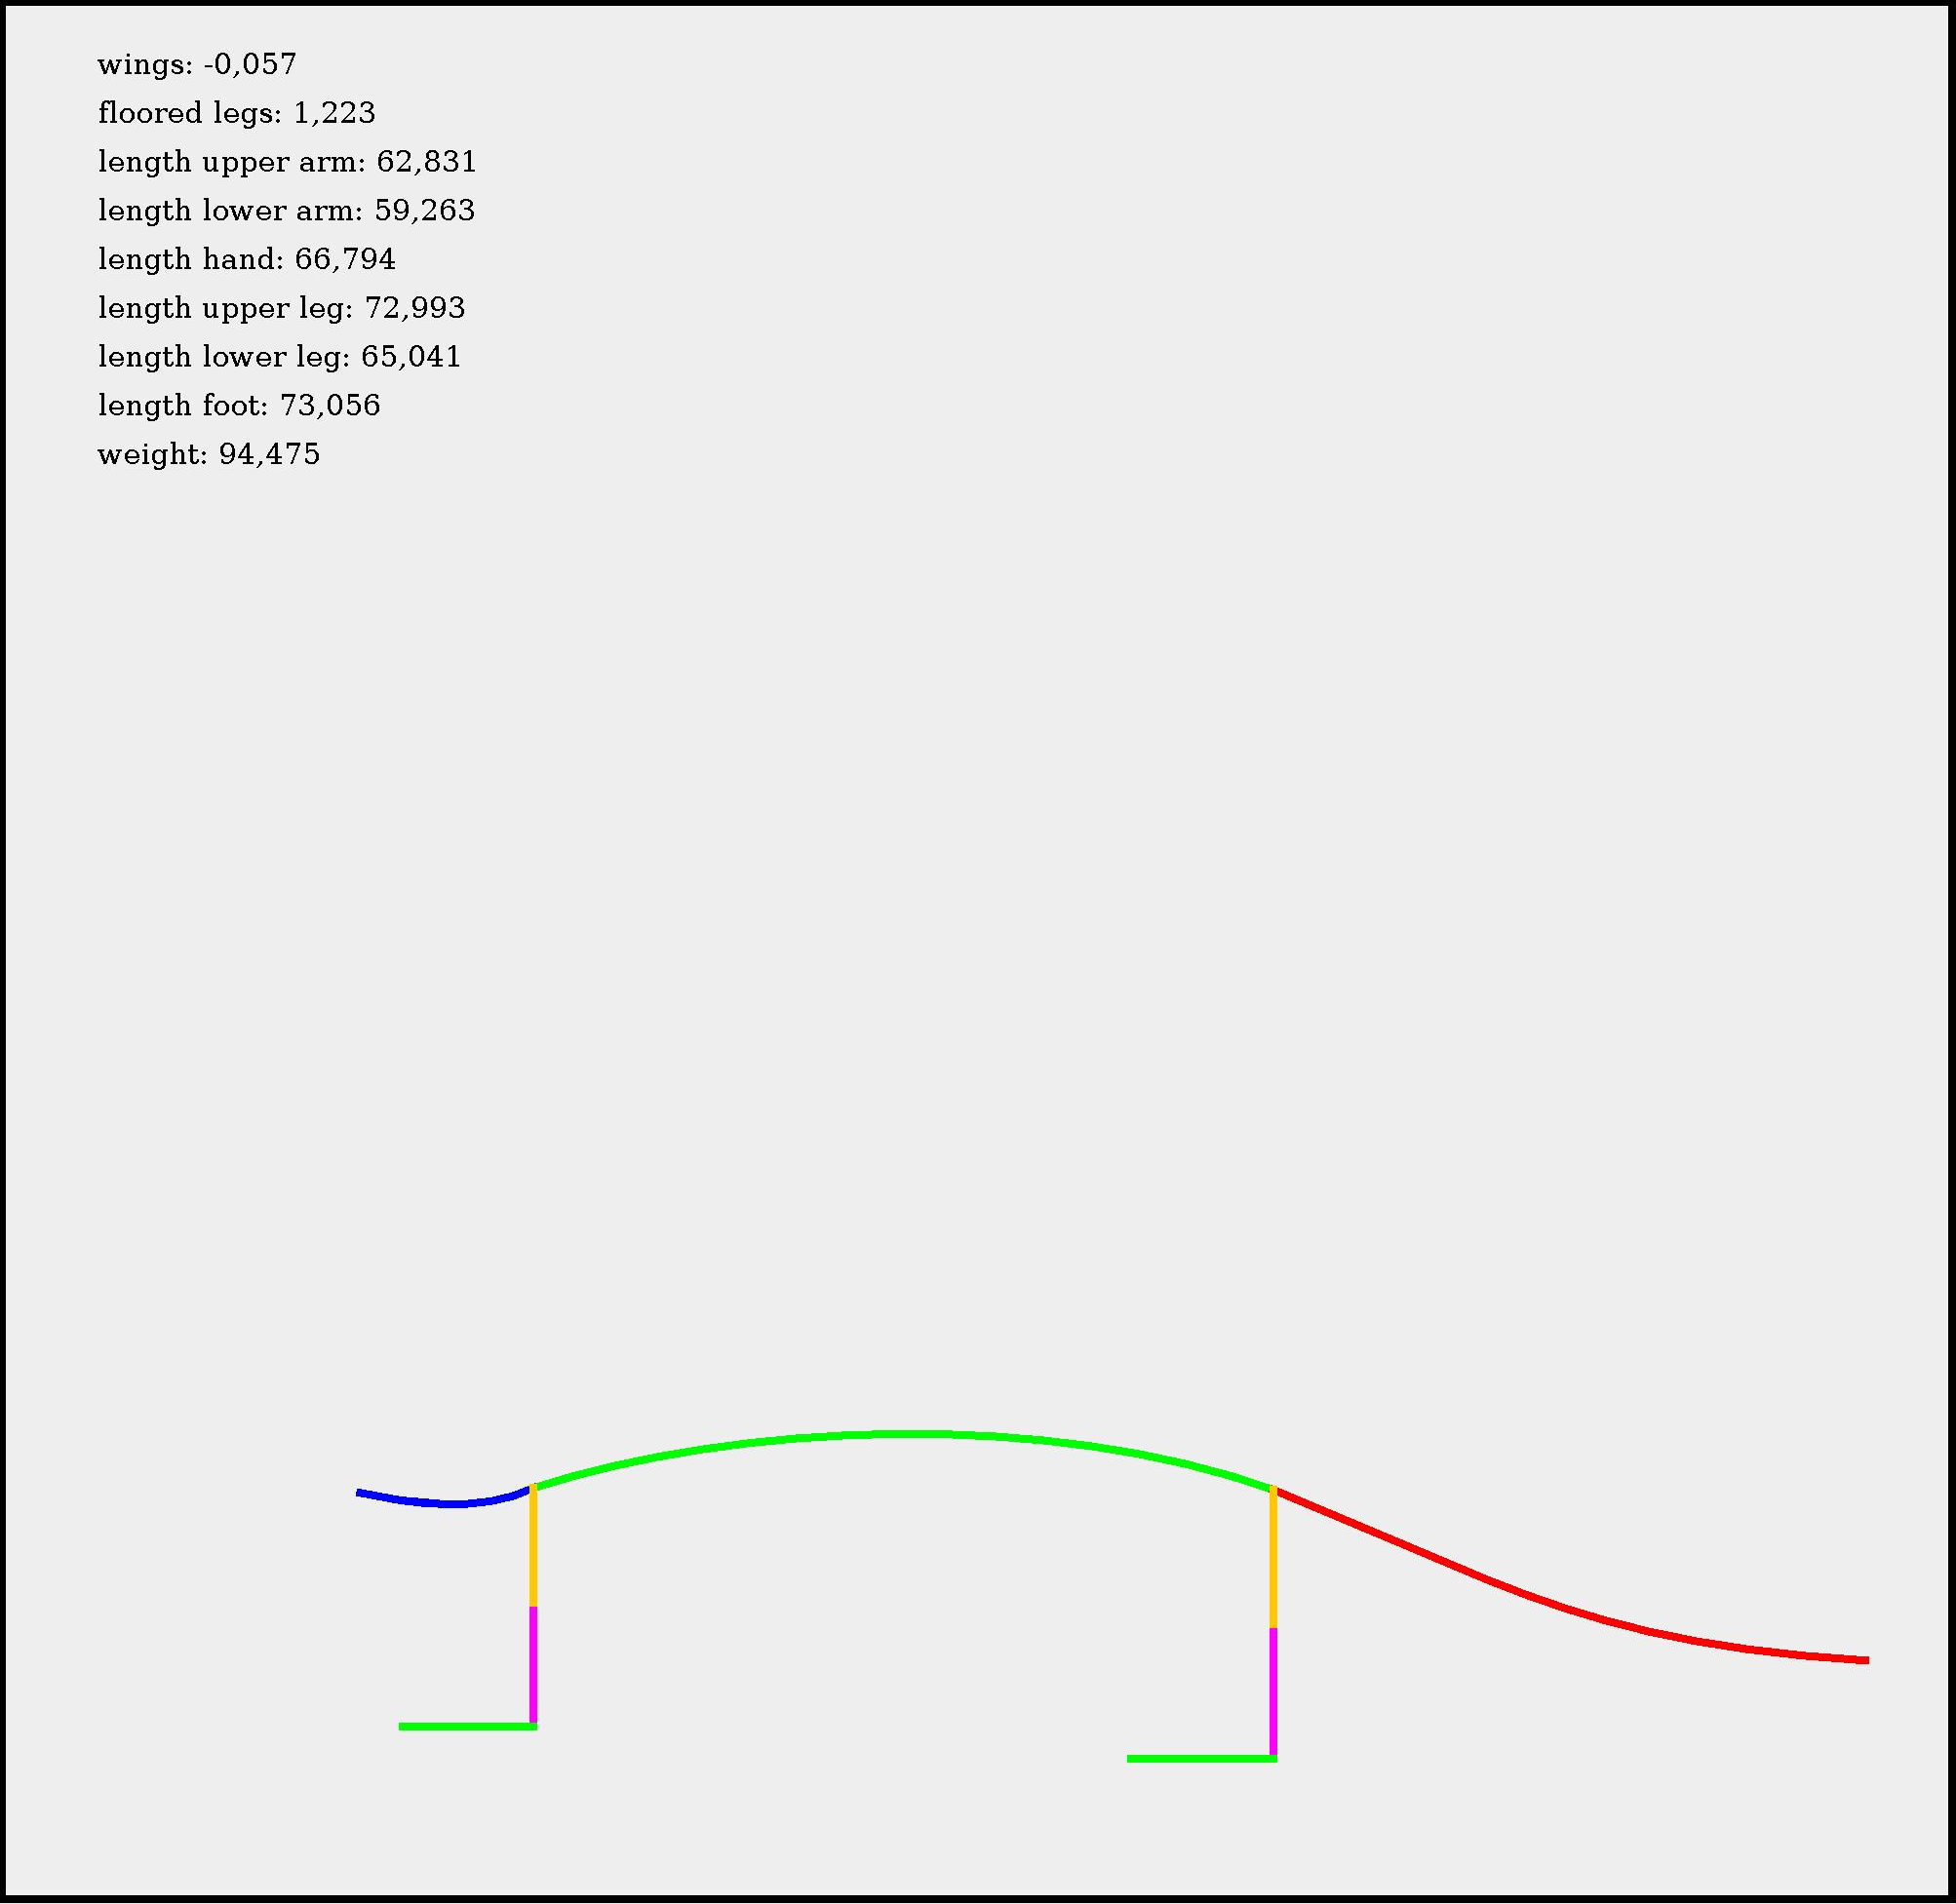
\includegraphics[height=0.5\textheight]{../../PCA/sqrtEV_log_weight_downscaled_wings_legs_and_weight/EV1_pos.jpg}}
  \caption{längste Achse: positive/negative Standardabweichung}
 \end{figure}
\end{frame}

%--------------------
\section{Der Algorithmus}
%--------------------
\begin{frame}{Überblick über den Algorithmus}
 \begin{enumerate}
  \setcounter{enumi}{-1}
  \item Benutzereingabe einlesen
  \item PCA auf Beispielskeletten durchführen
  \item[2a.] Punkt $q$ im Konfigurationsraum (zufällig) bestimmen 
  \item[2b.] Parameter für das Skelett aus $q$ und Benutzereingabe bestimmen
  \setcounter{enumi}{2}
  \item<2-> Bestandteile des Skeletts mit kontextfreier Grammatik $G$ erzeugen und positionieren
  \item<3-> Alle Knochen, die nicht auf der Wirbelsäule liegen, spiegeln
  \item<4-> 3D-Modell generieren
 \end{enumerate}
\end{frame}

\begin{frame}[focus]
 \begin{figure}
  \centering
  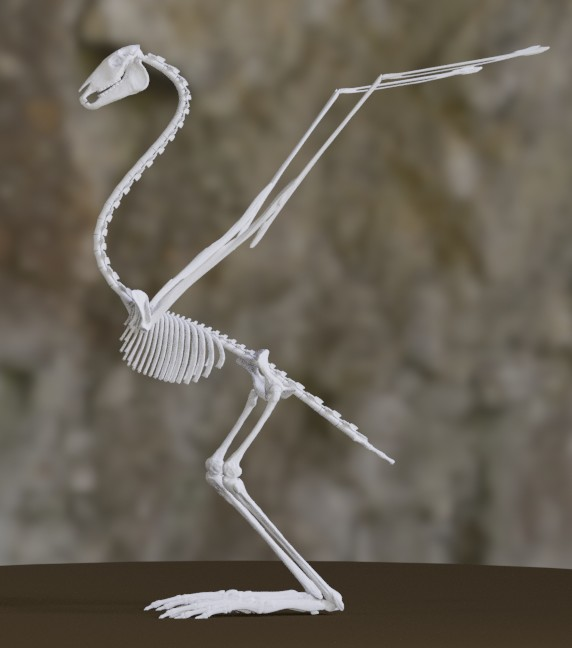
\includegraphics[height=0.9\textheight]{../../java_skeleton_generation/example_skeletons/bird.jpg}
 \end{figure}
\end{frame}

% Positionierung der Extremitäten

\begin{frame}[focus]
 \begin{figure}
  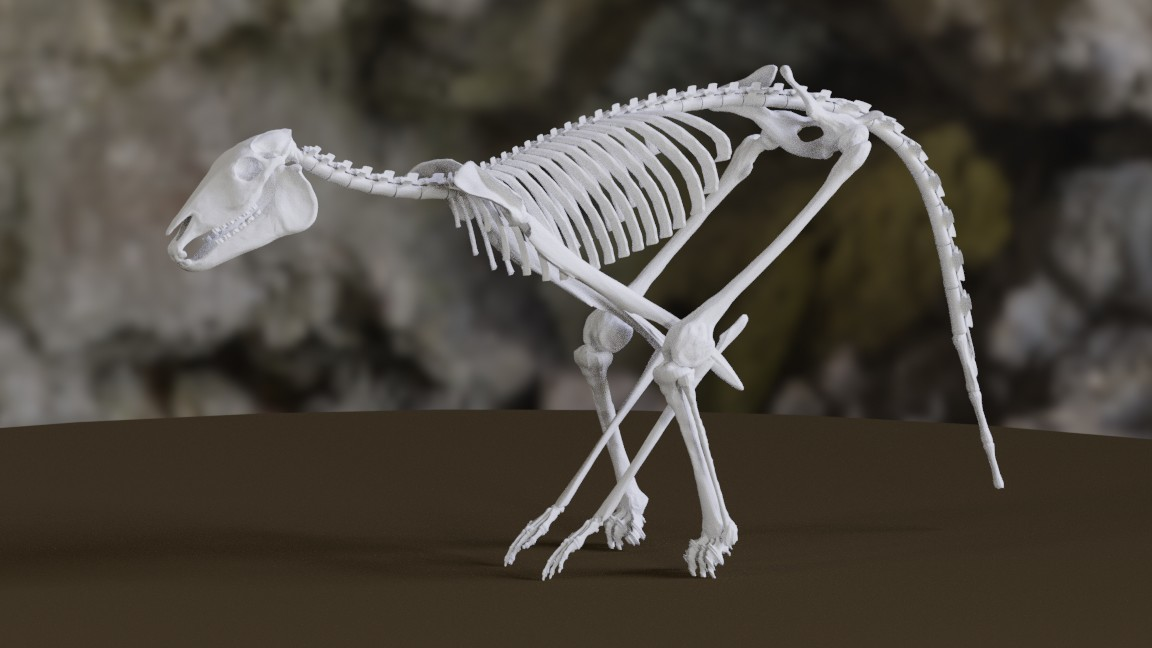
\includegraphics[width=\textwidth]{../../java_skeleton_generation/example_skeletons/elefant.jpg}
  \caption{Elefant}
 \end{figure}
\end{frame}

\begin{frame}[focus]
 \begin{figure}
  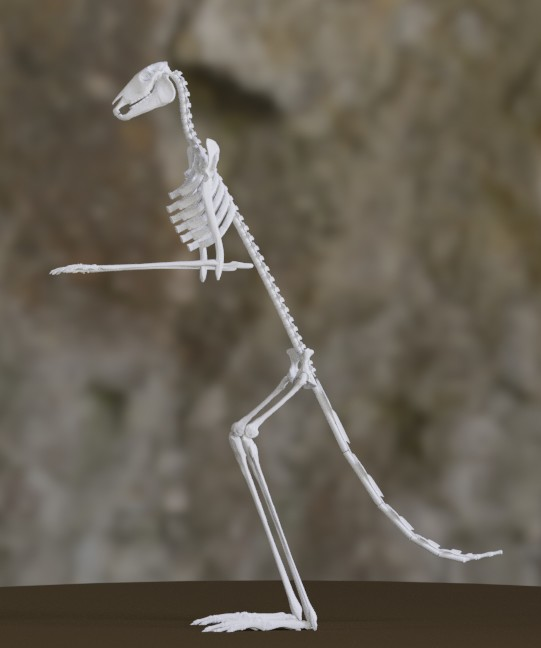
\includegraphics[height=0.85\textheight]{../../java_skeleton_generation/example_skeletons/kaenguru.jpg}
 \caption{Känguru}
 \end{figure}
\end{frame}

\begin{frame}[focus]
 \begin{figure}
  \centering
  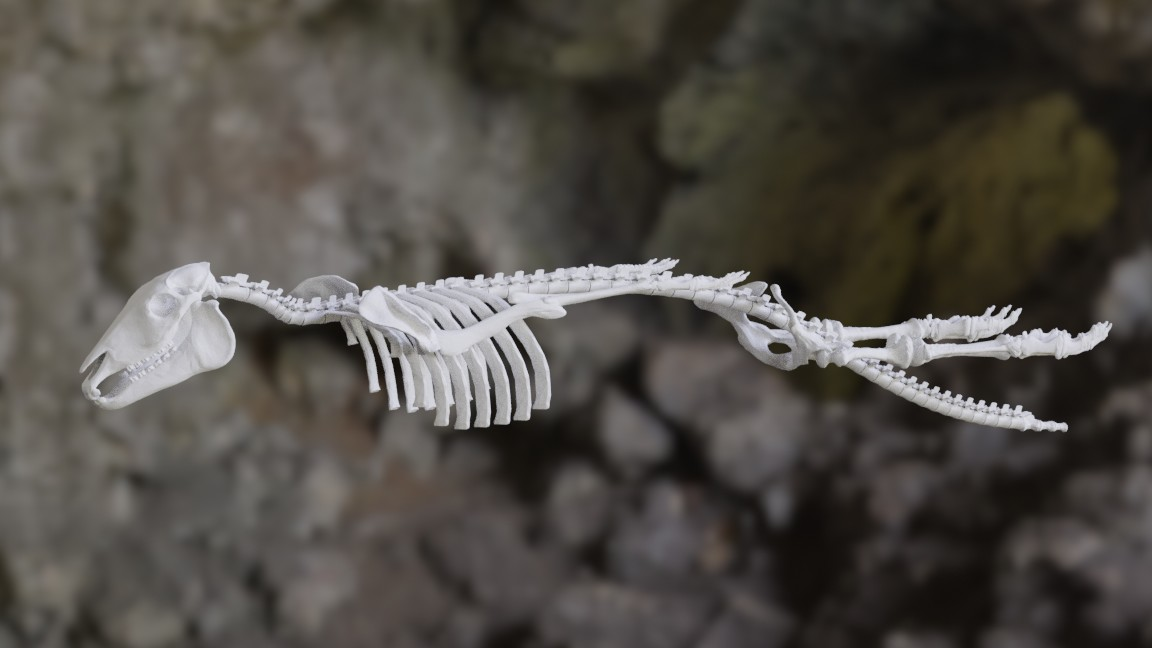
\includegraphics[width=\textwidth]{../../java_skeleton_generation/example_skeletons/fish.jpg}
 \end{figure}
\end{frame}

\begin{frame}[focus]
\begin{flushleft}
  \Large 3D-Modelle erstellen
 \end{flushleft}
 \vfill
 \begin{figure}
  \centering
  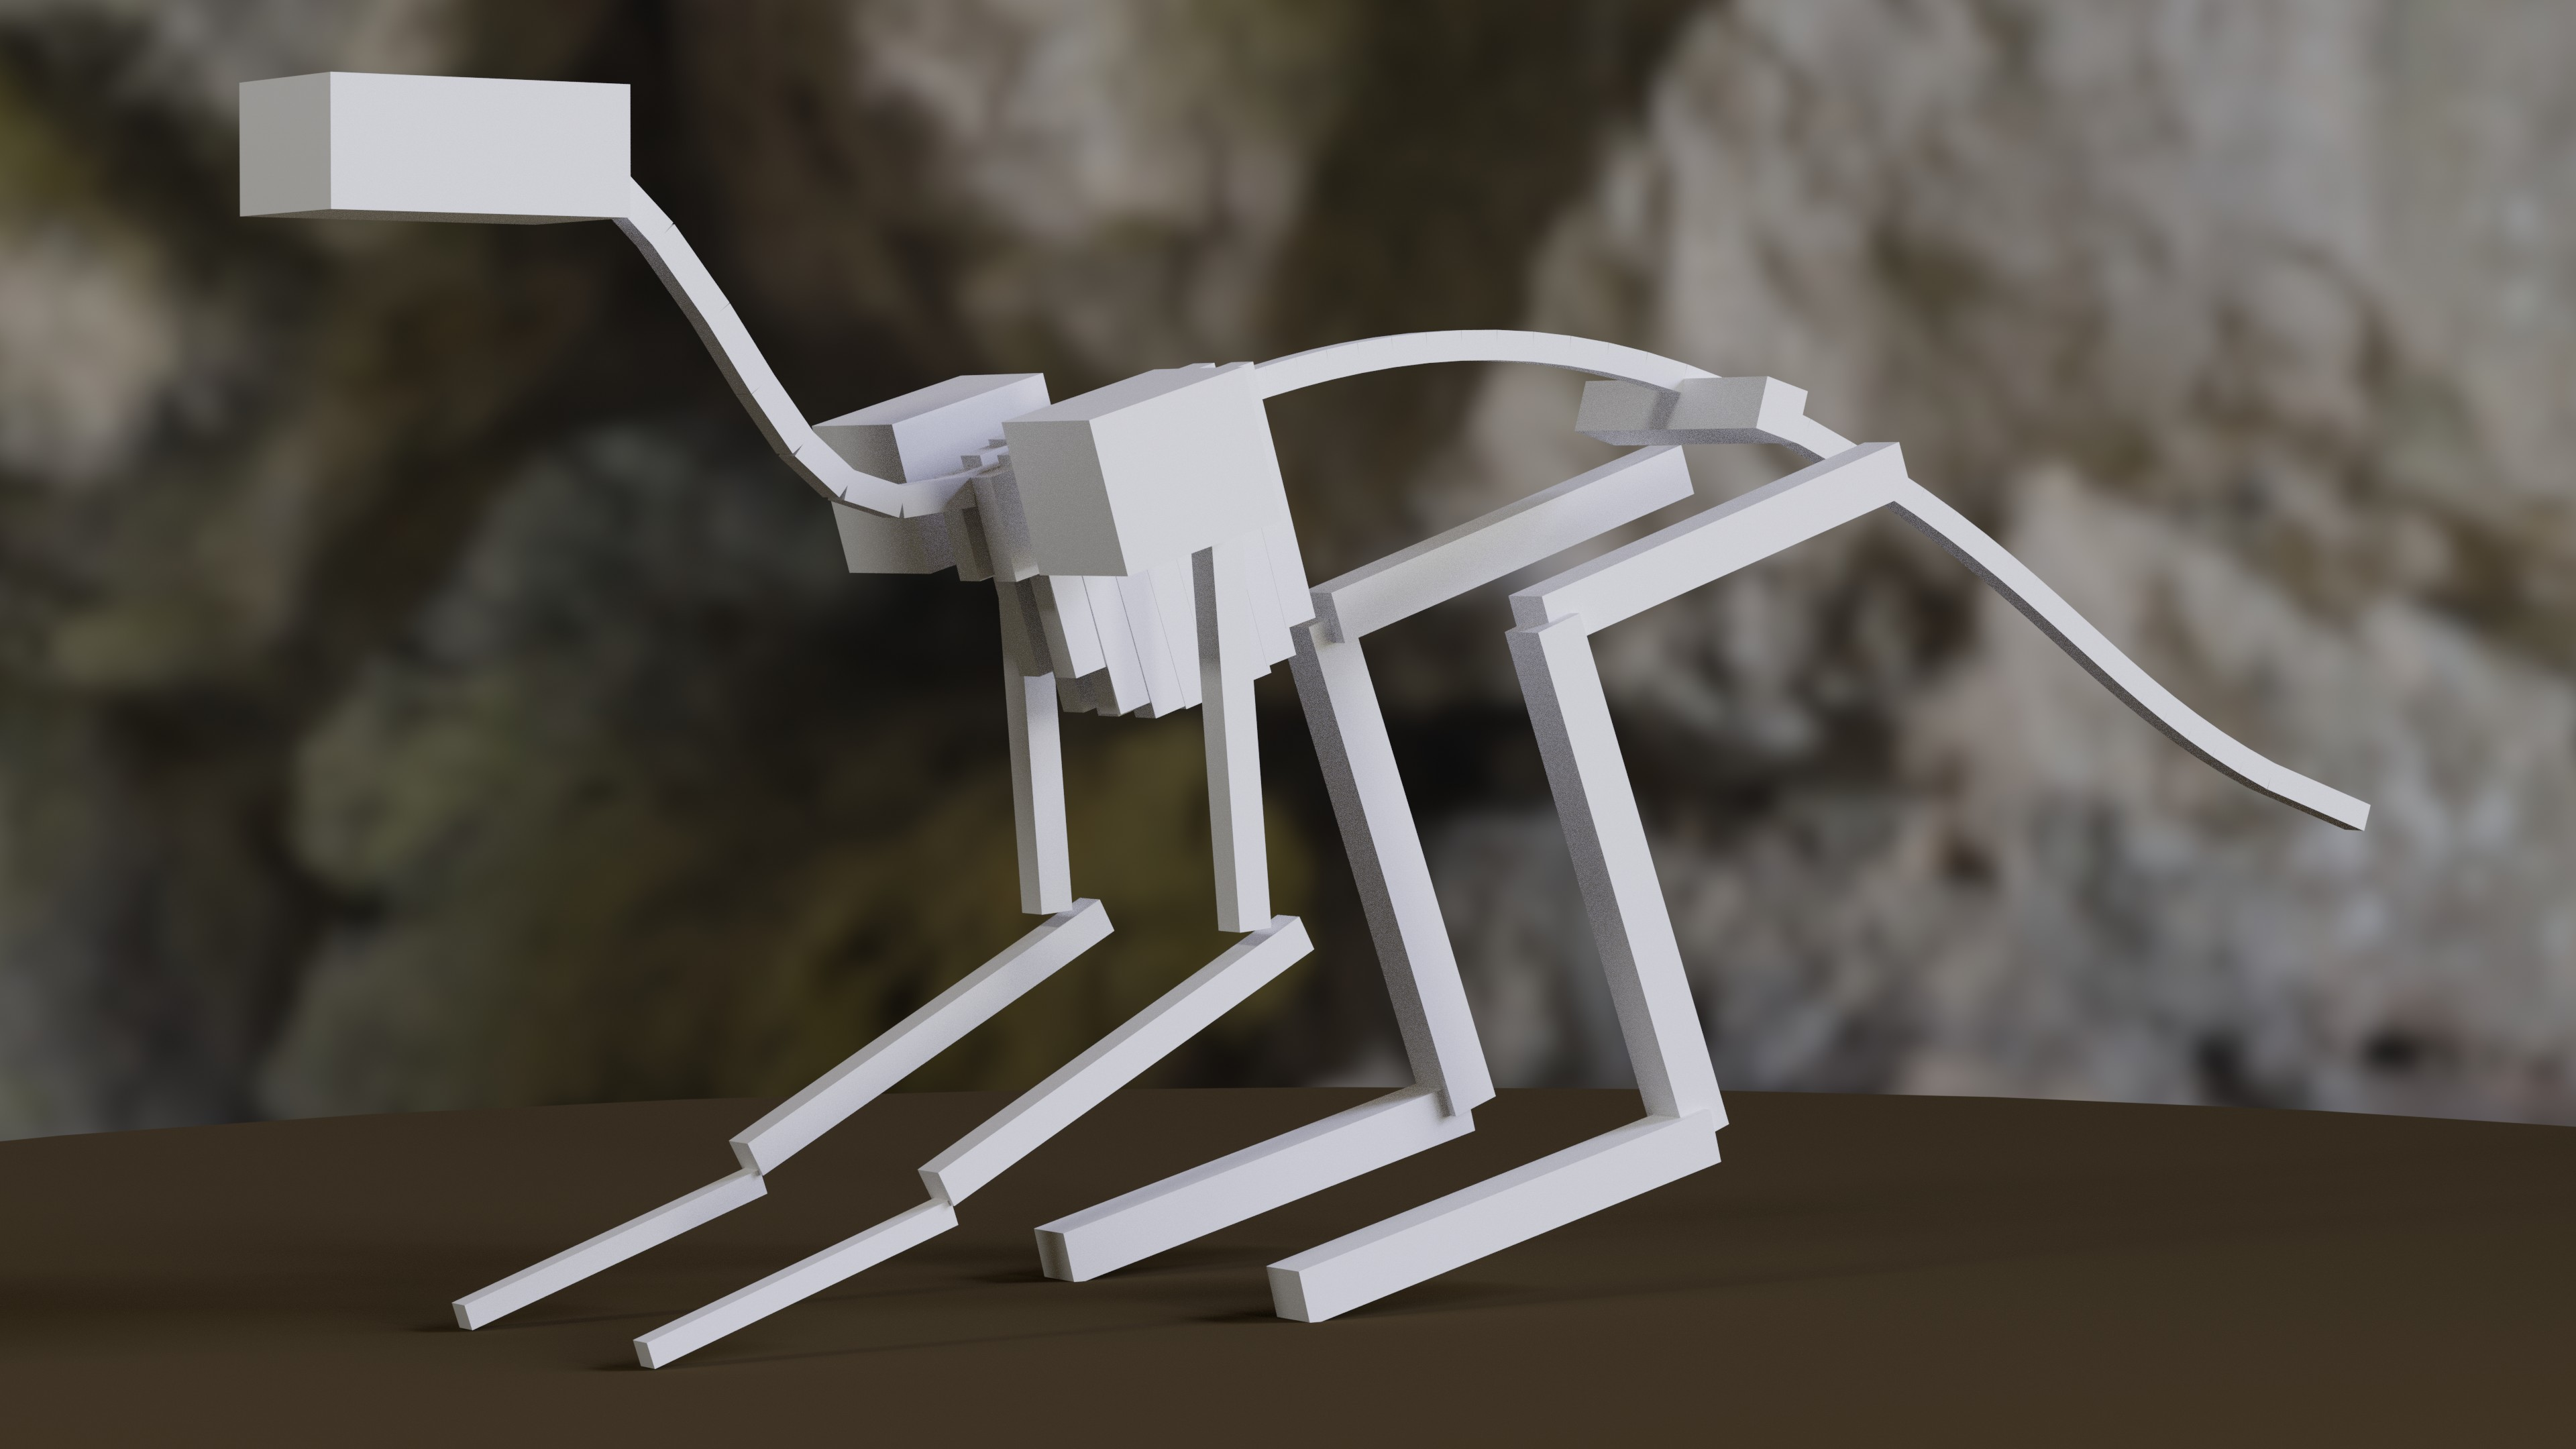
\includegraphics[width=\textwidth]{../../java_skeleton_generation/example_skeletons/4legs_boxes.jpg}
 \end{figure}
\end{frame}

\addtocounter{framenumber}{5}
\begin{frame}{Bedingungen}
 \begin{enumerate}
  \item Vorgegebene Punkte aus Konfigurationsraum laden\\ (\zb Eingabebeispiele)
  \item Bedingte Verteilung als Eingabe für PCA
  \begin{itemize}
   \item explizite Merkmale (\zb Anzahl Flügel und Beine)
   \item implizite Merkmale (\zb Länge des Schwanzes in $x$-Richtung)
  \end{itemize}
  \item Schon einmal generierte Skelette laden
 \end{enumerate}
 \begin{block}<2>{Variationen}
  \begin{itemize}
   \item Gegeben: Punkt $q$ im Konfigurationsraum
   \item Bestimme Punkt $q'$ zufällig normalverteilt mit Erwartungswert $q$
  \end{itemize}
 \end{block}
\end{frame}

%---------------------------
\section{Fantastische Tiere}
%---------------------------

\begin{frame}[focus]
 \begin{flushleft}
  \Large Pegasus -- $2$ Extremitätenpaare pro Gürtel
 \end{flushleft}
 \vfill
 \begin{figure}
  \centering
  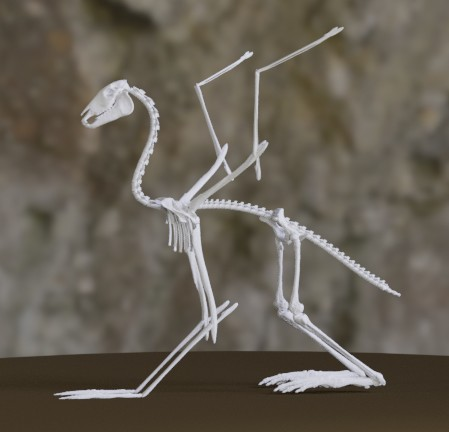
\includegraphics[height=0.75\textheight]{../../java_skeleton_generation/example_skeletons/pegasus.jpg}
 \end{figure}
\end{frame}

\begin{frame}[focus]
 \begin{flushleft}
  \Large Zentaur -- Zweiter Schultergürtel
 \end{flushleft}
 \vfill
 \begin{figure}
  \centering
  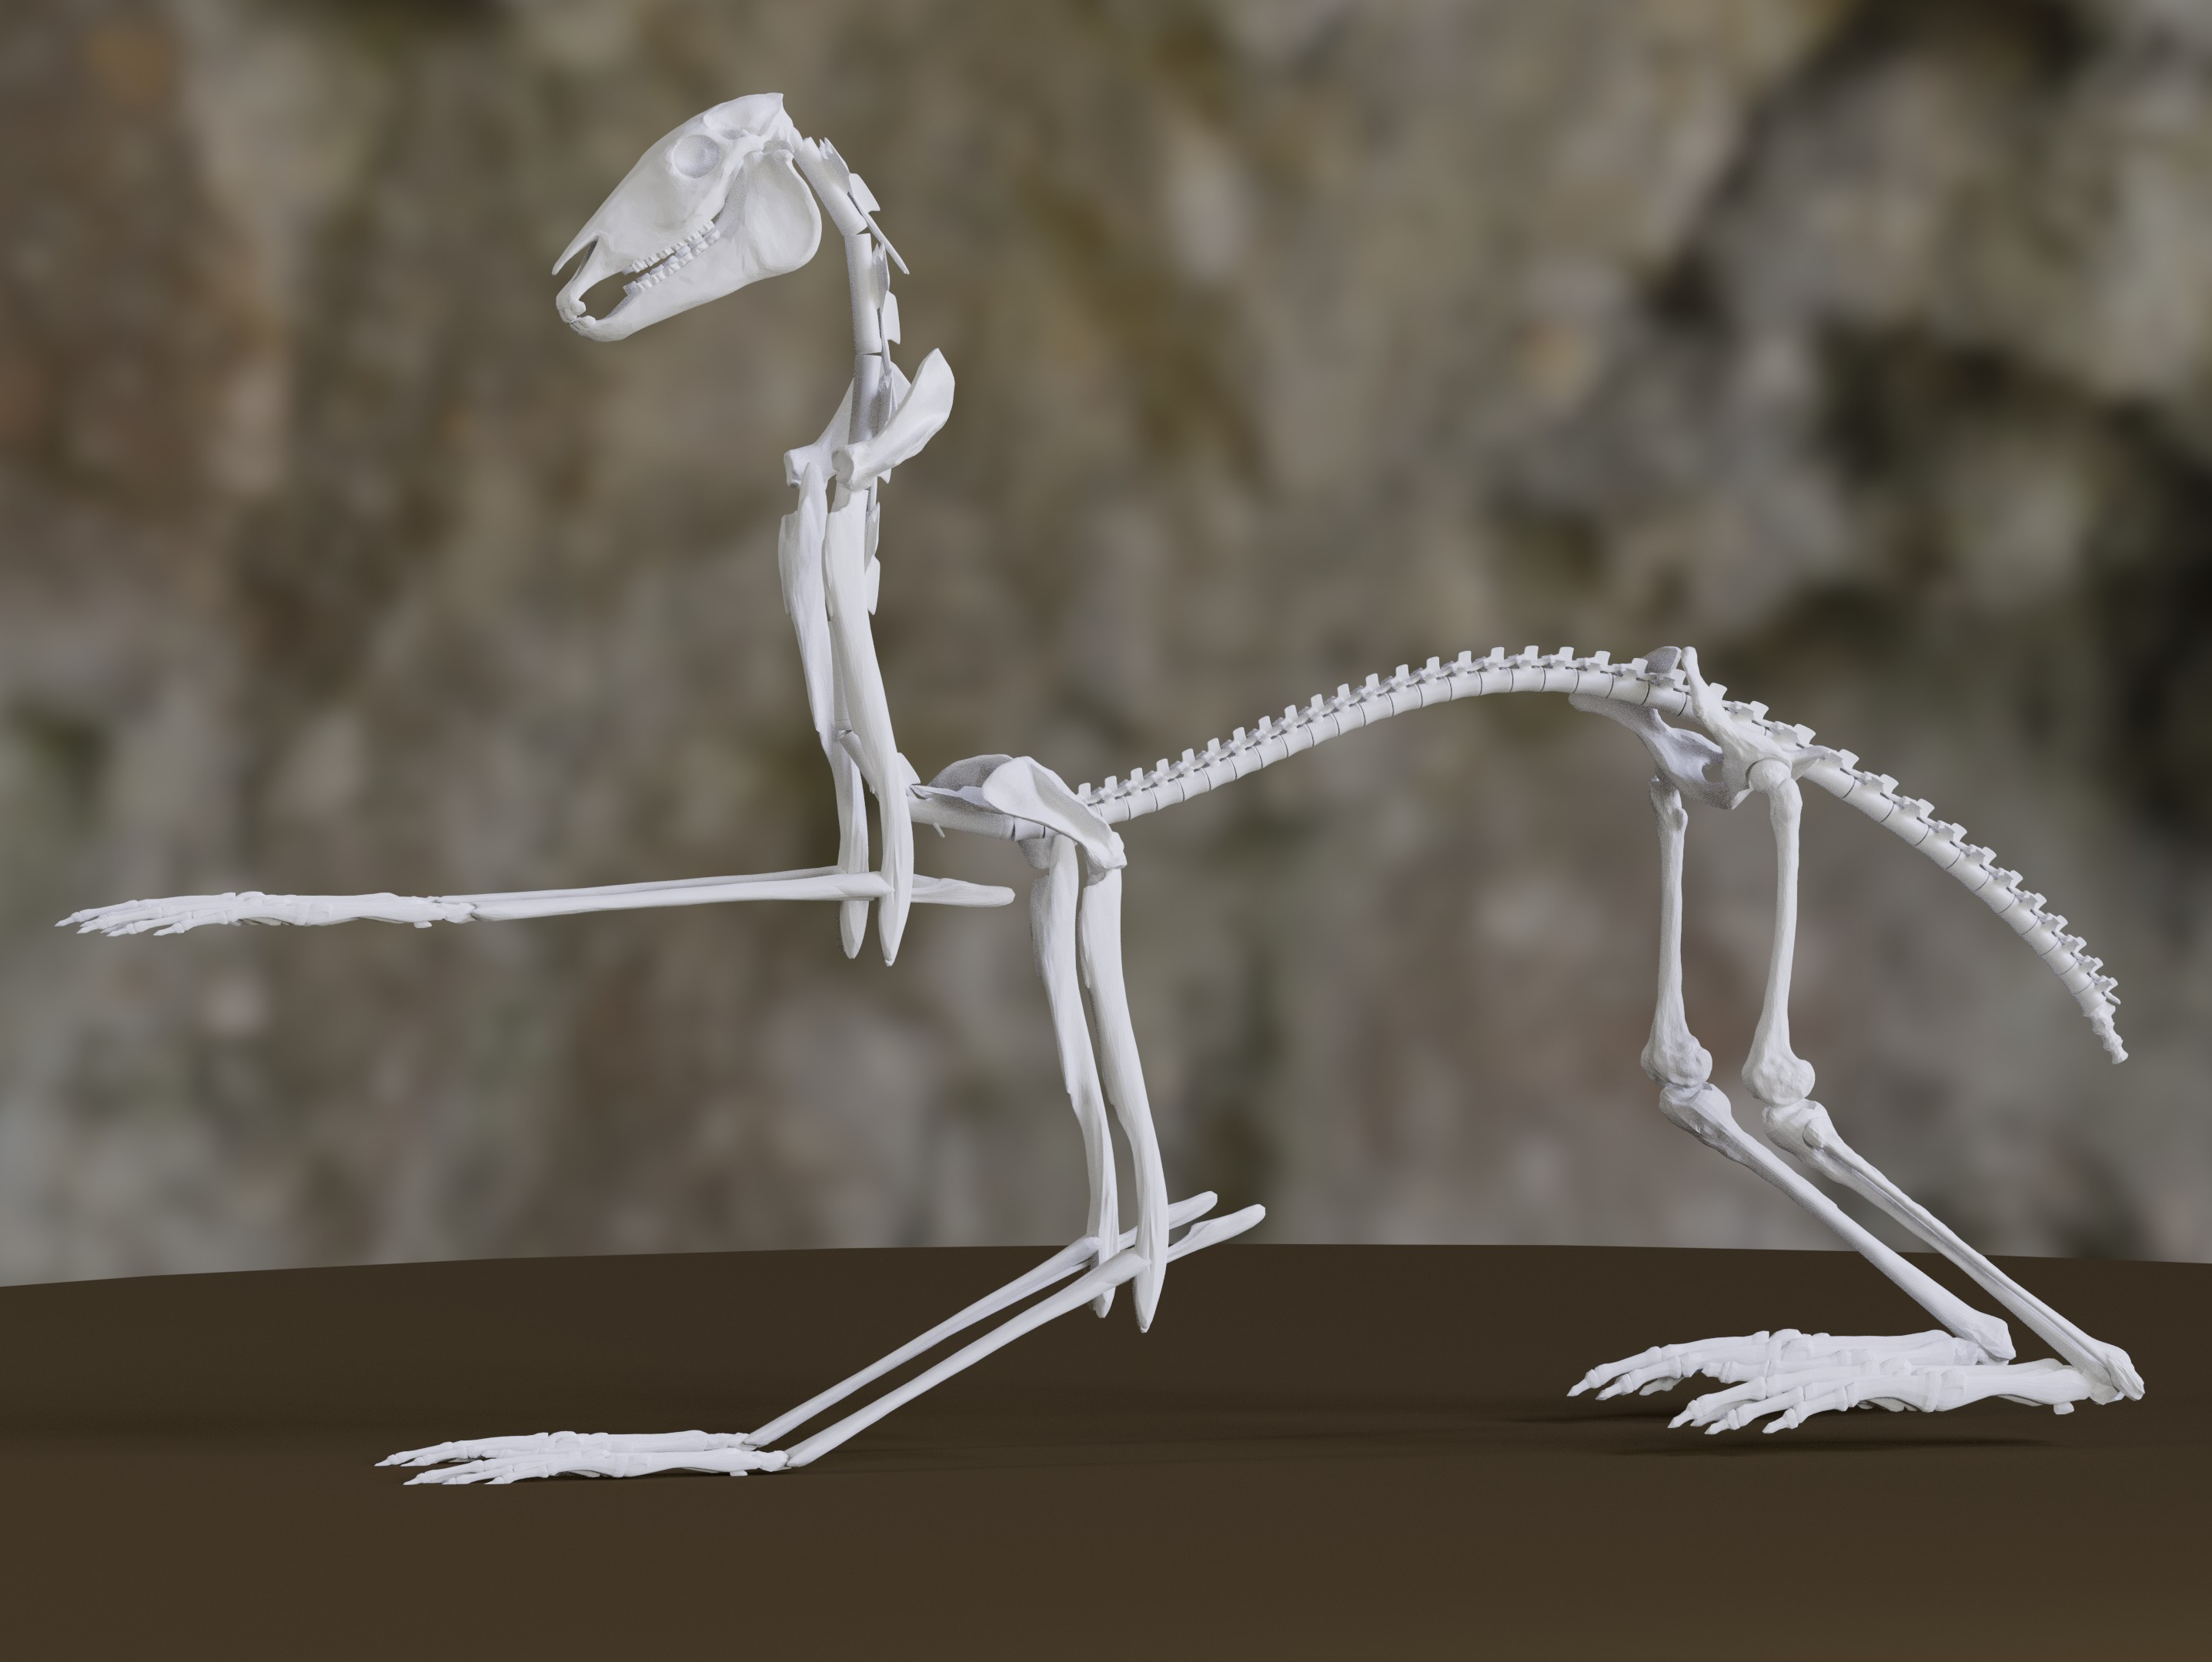
\includegraphics[height=0.75\textheight]{../../java_skeleton_generation/example_skeletons/zentaur2.jpg}
 \end{figure}
\end{frame}

\addtocounter{framenumber}{2}

\begin{frame}{Ausblick}
 \begin{itemize}
  \item Auch Skelette mit sehr aufrechter Wirbelsäule wie beim Menschen generierbar?
  \item Wert des Gewichts der Tiere verwenden \zb als Einfluss auf die Größe der Tiere oder die Dicke ihrer Knochen
  \item mehr verschiedene und leichter austauschbare Knochenmodelle
  \item interaktiver Algorithmus
  \item Muskeln und Haut generieren
 \end{itemize}
\end{frame}


\begin{frame}[focus]
 Vielen Dank für die Aufmerksamkeit!
 \vfill
 \small weitere Informationen unter \url{https://github.com/Zimmt/skeleton-generation}
\end{frame}

\appendix
\begin{frame}[shrink=5]{Quellen}
 \printbibliography[heading=bibintoc]
\end{frame}

\begin{frame}{Untersuchung auf Normalverteilung}
 Quantil-Quantil-Diagramme
  \begin{figure}
  \subfloat[x-Wert der $3$. Koordinate des Halses]{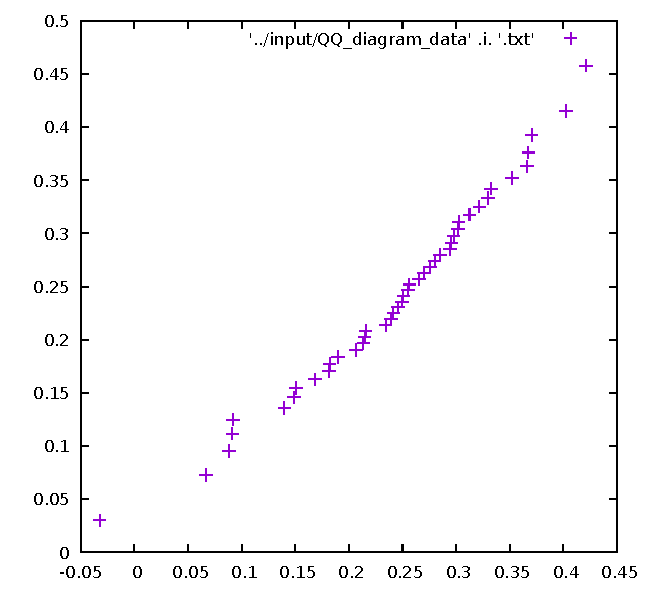
\includegraphics[width=0.3\textwidth]{../../PCA/gnuplot/results_qq_diagrams/QQ_diagram4.pdf}}~
  \subfloat[Länge der Hand]{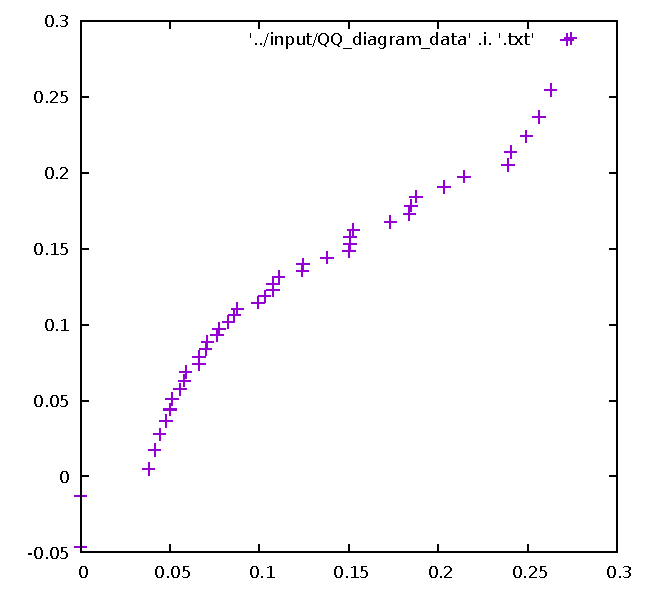
\includegraphics[width=0.3\textwidth]{../../PCA/gnuplot/results_qq_diagrams/QQ_diagram24.pdf}}~
  \subfloat[Länge des Oberschenkels]{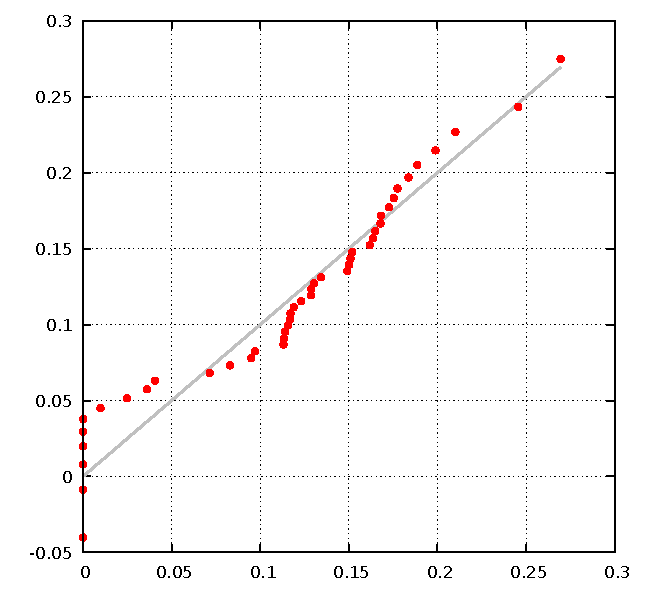
\includegraphics[width=0.3\textwidth]{../../PCA/gnuplot/results_qq_diagrams/QQ_diagram25.pdf}}
  \phantomcaption
 \end{figure}
\end{frame}

\begin{frame}{Normalverteilung des Gewichts}
 \centering
 \begin{figure}
  \subfloat[linear]{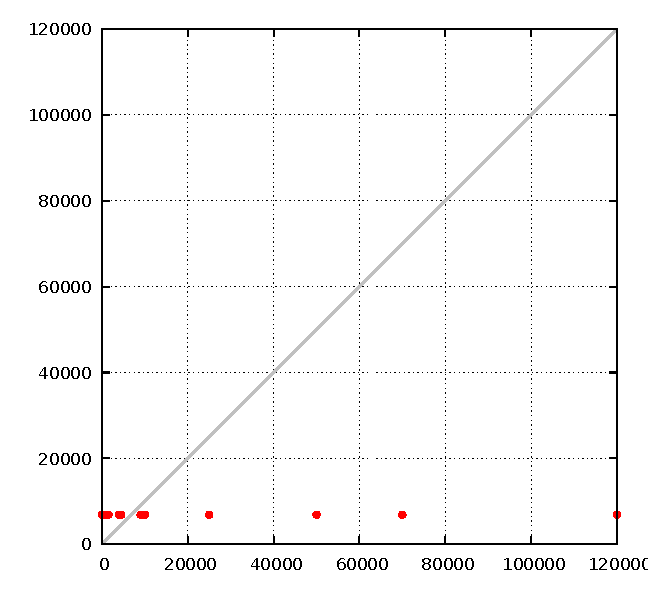
\includegraphics[width=0.3\textwidth]{../../PCA/gnuplot/results_qq_diagrams/QQ_diagram_linear_weight.pdf}}~
  \subfloat[linear (Ausschnitt)]{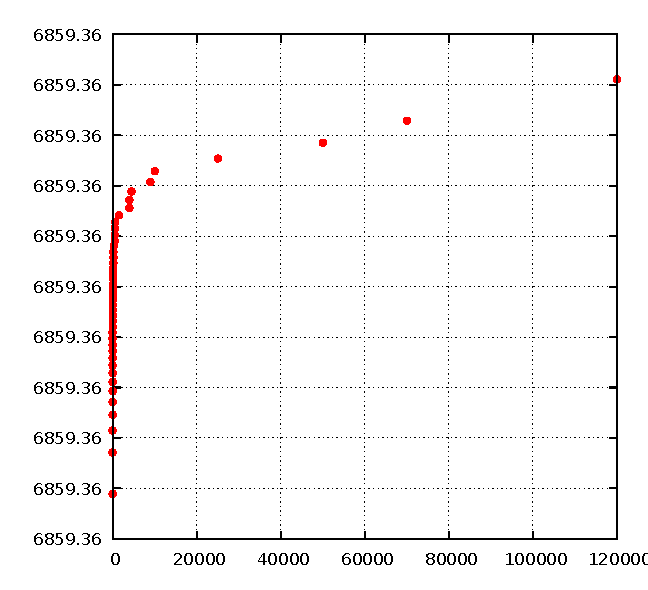
\includegraphics[width=0.3\textwidth]{../../PCA/gnuplot/results_qq_diagrams/QQ_diagram_linear_weight_without_diagonal.pdf}}~
  \subfloat[logarithmisch]{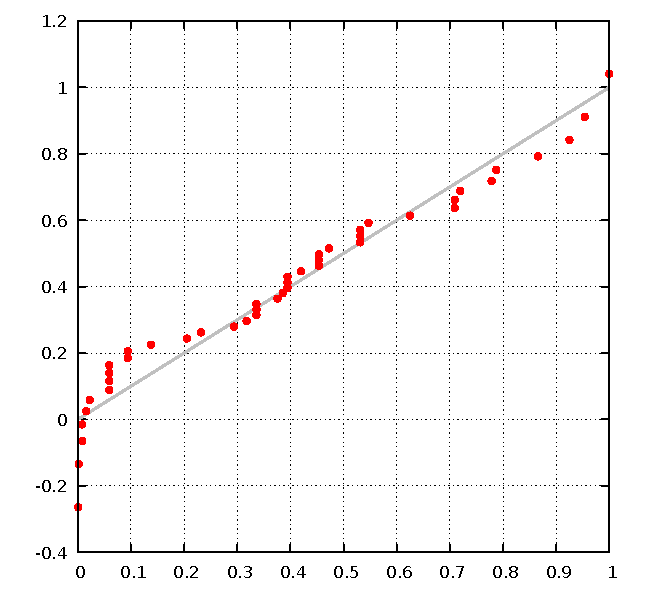
\includegraphics[width=0.3\textwidth]{../../PCA/gnuplot/results_qq_diagrams/QQ_diagram28.pdf}}
  \phantomcaption
 \end{figure}
 $\Rightarrow$ Das logarithmische Gewicht wird verwendet.
\end{frame}

\begin{frame}{Gewichtung der Merkmale}
 \begin{itemize}
  \item Alle Merkmale zunächst auf $[0, 1]$ skaliert
  \item Diskrete Merkmale (Anzahl Flügel und Beine) nicht normalverteilt, liefern aber hilfreiche Informationen $\rightarrow$ kleiner skalieren
  \item Gewicht nicht Hauptmerkmal $\rightarrow$ kleiner skalieren
 \end{itemize}
\end{frame}

\begin{frame}{Analyse der Eingabedaten}
  \begin{figure}
  \subfloat{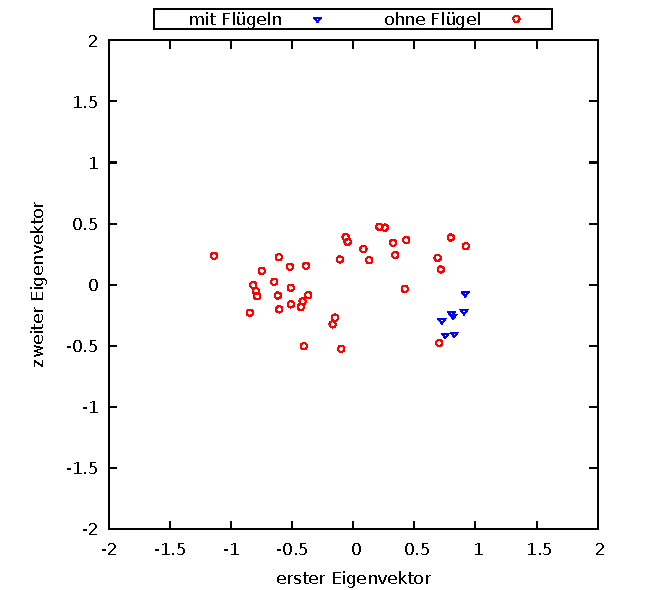
\includegraphics[width=0.5\textwidth]{../../PCA/gnuplot_log_weight_with_downscaled_wings_legs_and_weight/results_with_wing_tag/projection_eigenvectors12.pdf}}~
  \subfloat{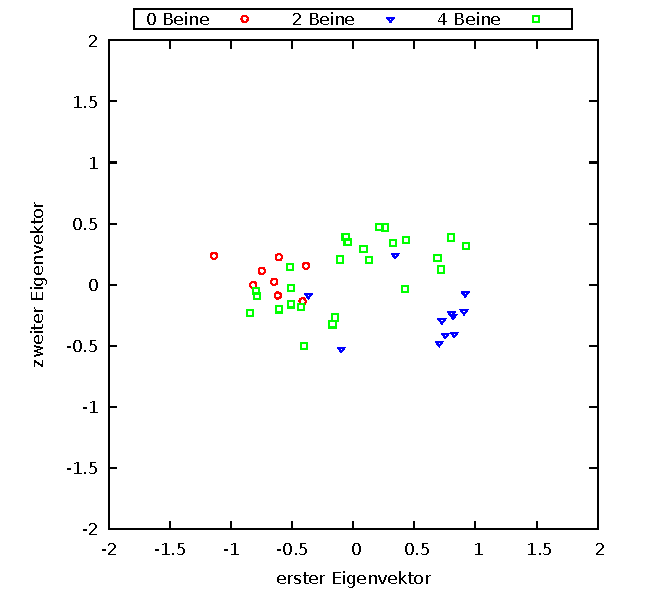
\includegraphics[width=0.5\textwidth]{../../PCA/gnuplot_log_weight_with_downscaled_wings_legs_and_weight/results_with_leg_tag/projection_eigenvectors12.pdf}}
  
  \caption{Projektion der Eingabedaten auf die Ebene, die durch die erste und zweite Achse des Hyperellipsoids aufgespannt wird.}
 \end{figure}
\end{frame}

\begin{frame}{Reduzierung der Dimensionalität mit PCA}
  \begin{figure}
  \centering
  \subfloat[Rekonstruktion aus 6 Eigenvektoren]{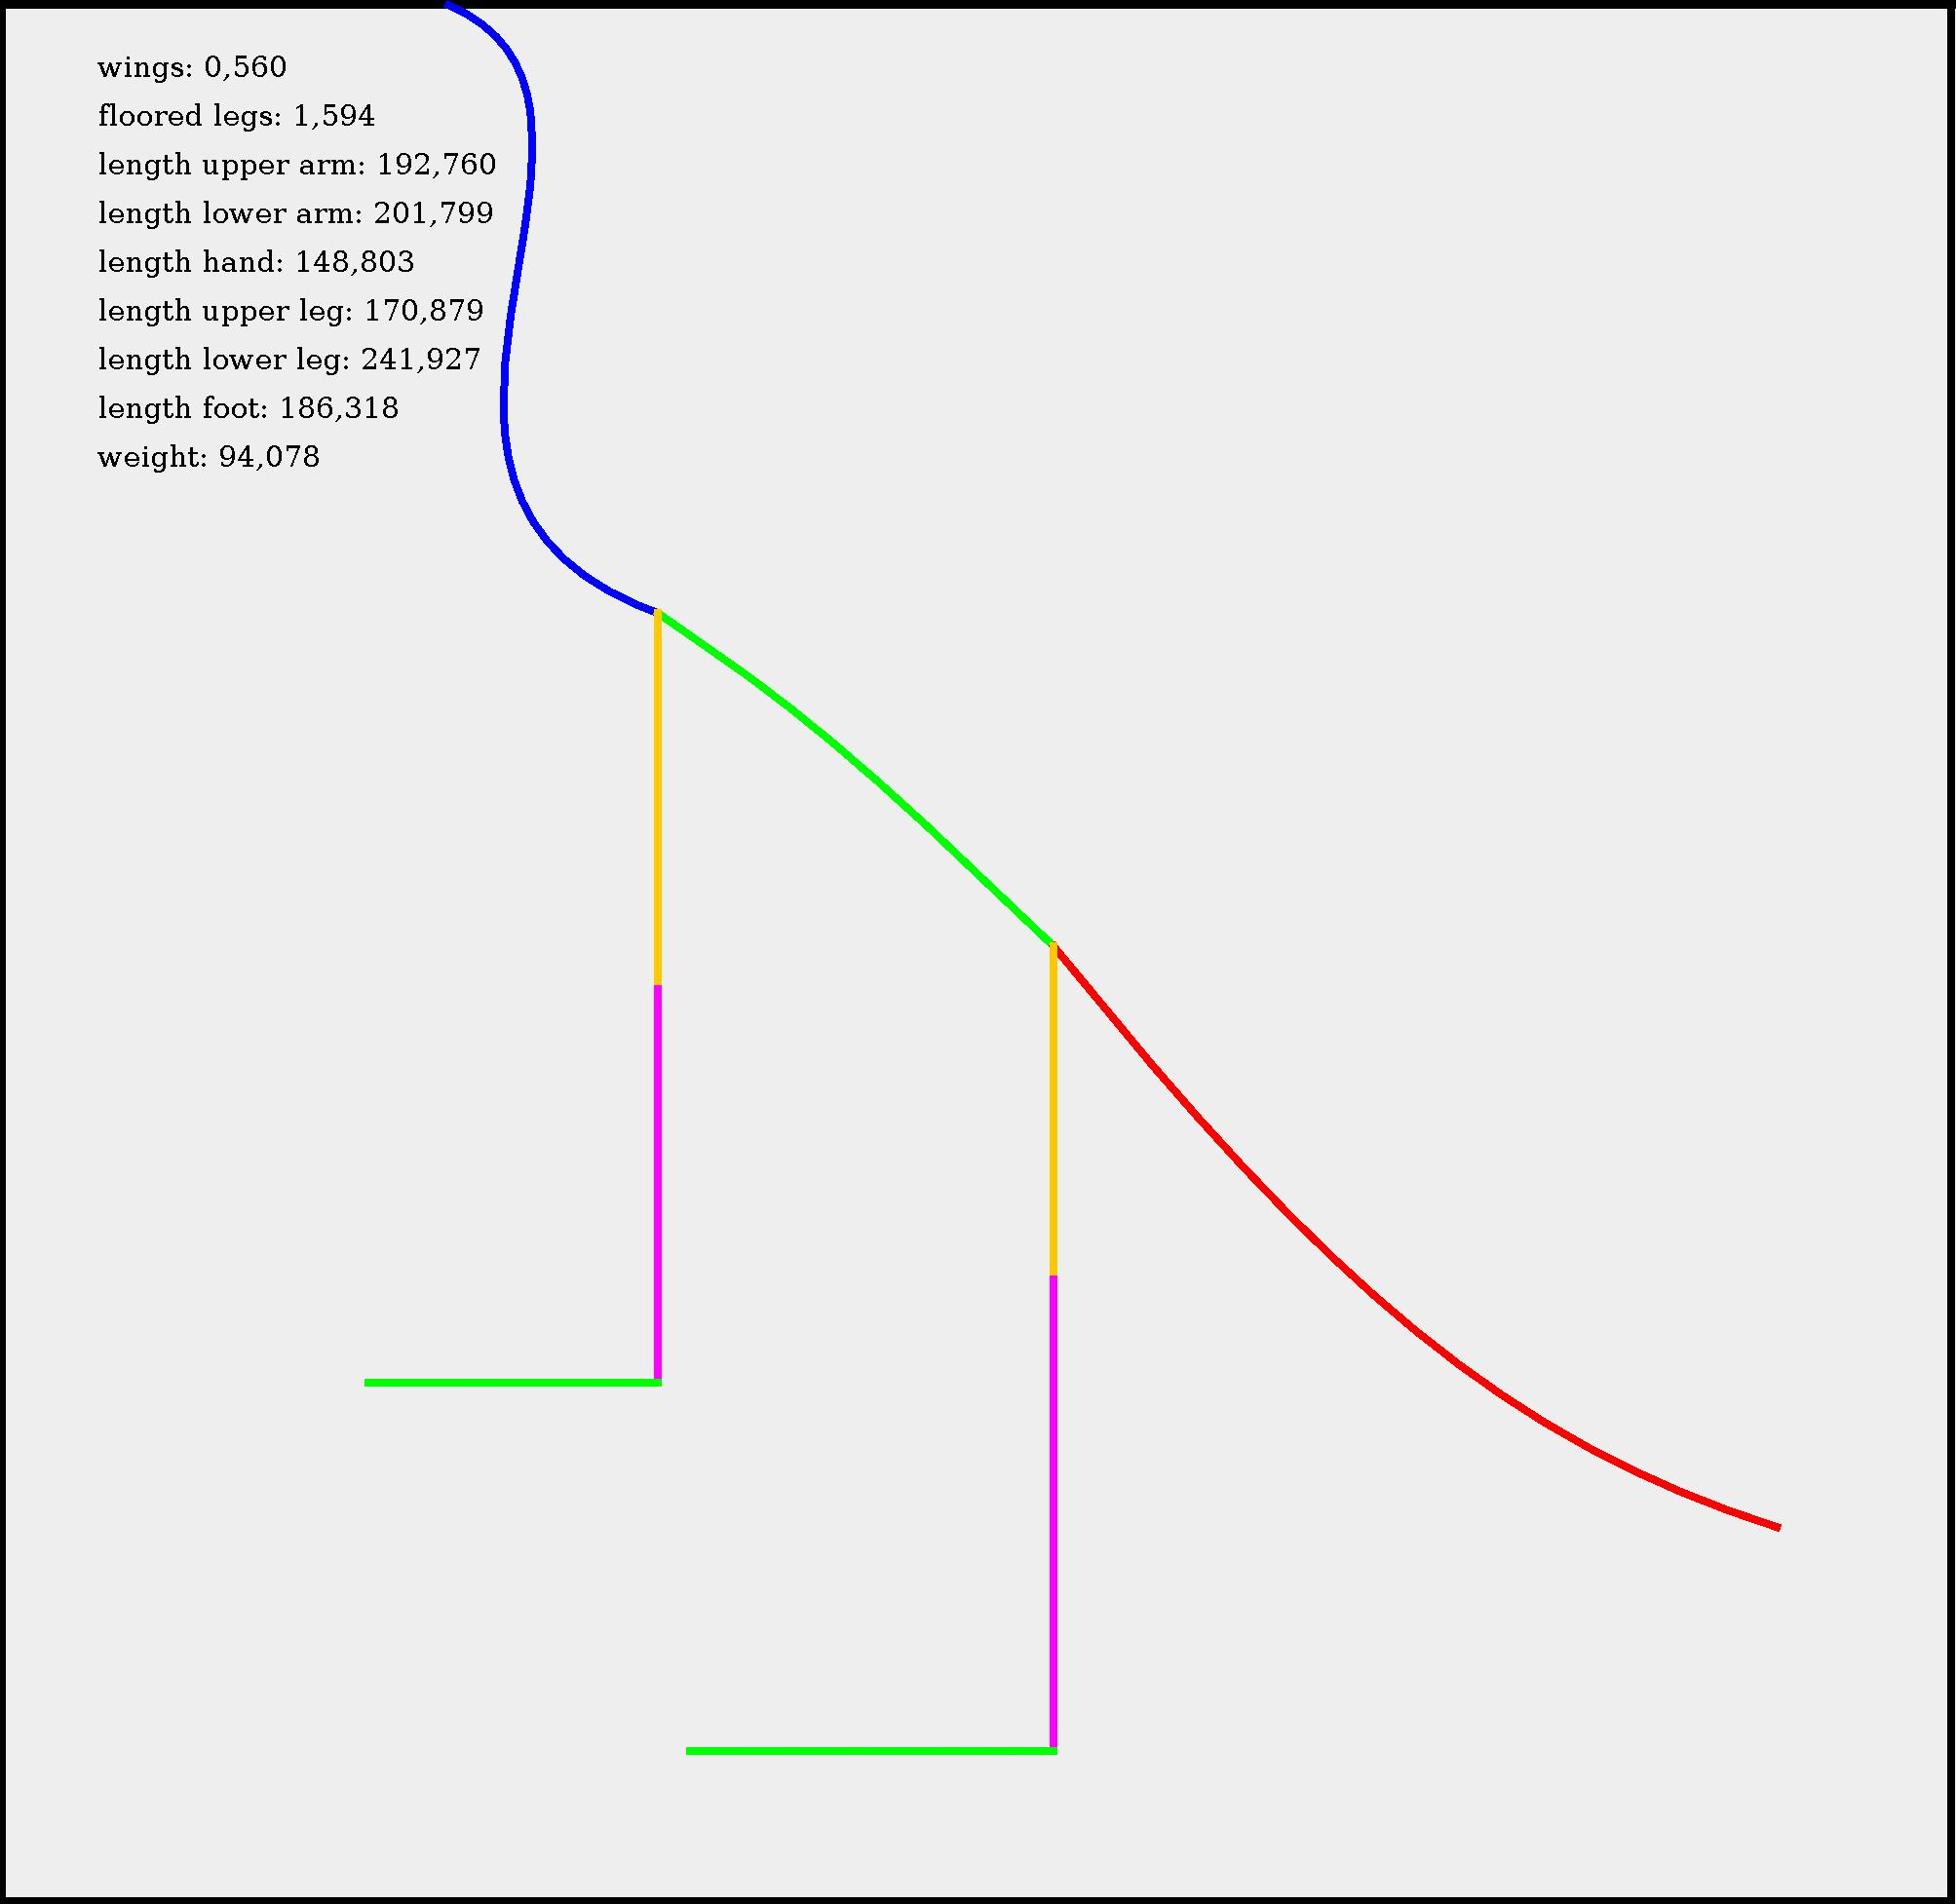
\includegraphics[width=0.4\textwidth]{../../PCA/animal_reconstructions_log_weight_downscaled_wings_legs_and_weight/6EV/Archaeopteryx_Ausschnitt.jpg}}~
  \subfloat[Eingabebild \cite{Zoologie24Wehner}]{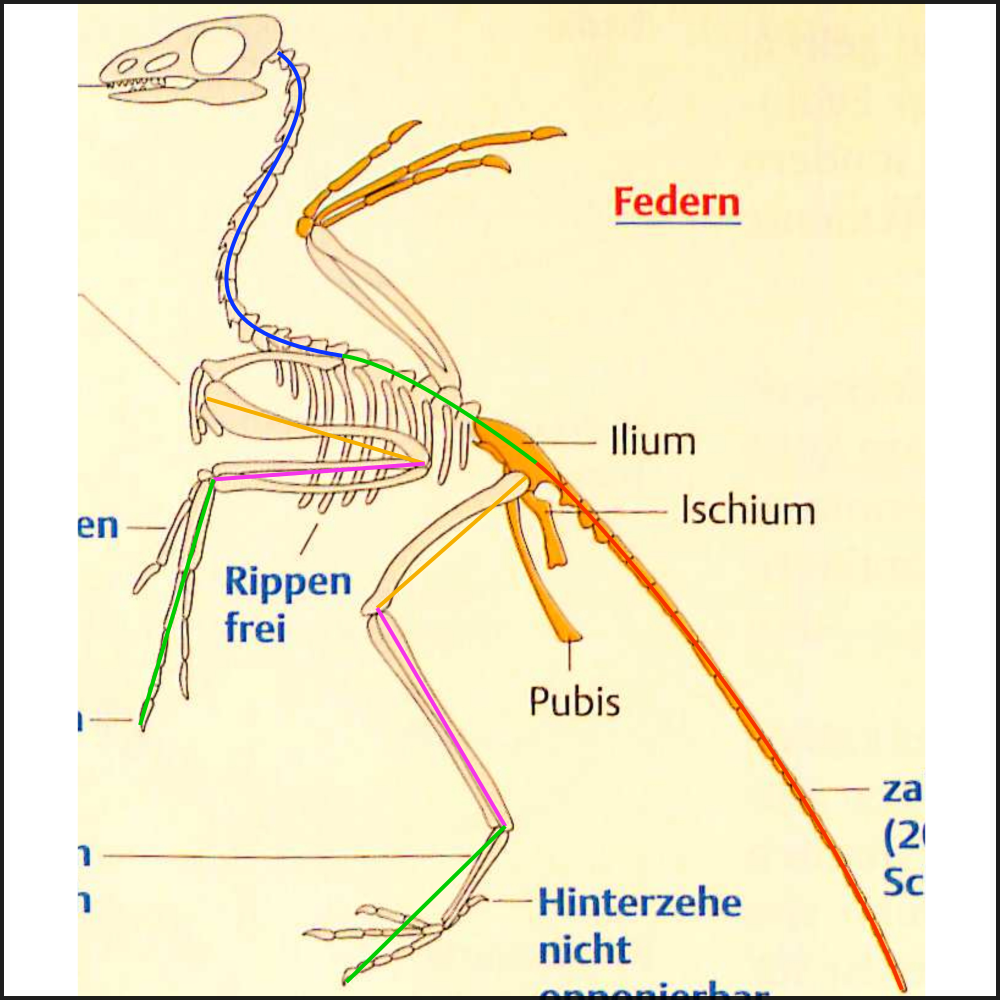
\includegraphics[width=0.4\textwidth]{../../PCA/Skelettbilder/Archaeopteryx_farbig.png}}
  
  \caption{Nicht visualisierte Daten der Rekonstruktion: \emph{Flügel} $0{,}56$, \emph{Beine mit Bodenkontakt} $1{,}594$, \emph{Gewicht}~$94{,}1$kg; Originalwert für das \emph{Gewicht}: $1$kg}
 \end{figure}
\end{frame}

\begin{frame}{Reduzierung der Dimensionalität mit PCA}
 \begin{figure}
  \centering
  \subfloat[Rekonstruktion aus $6$ Eigenvektoren]
  {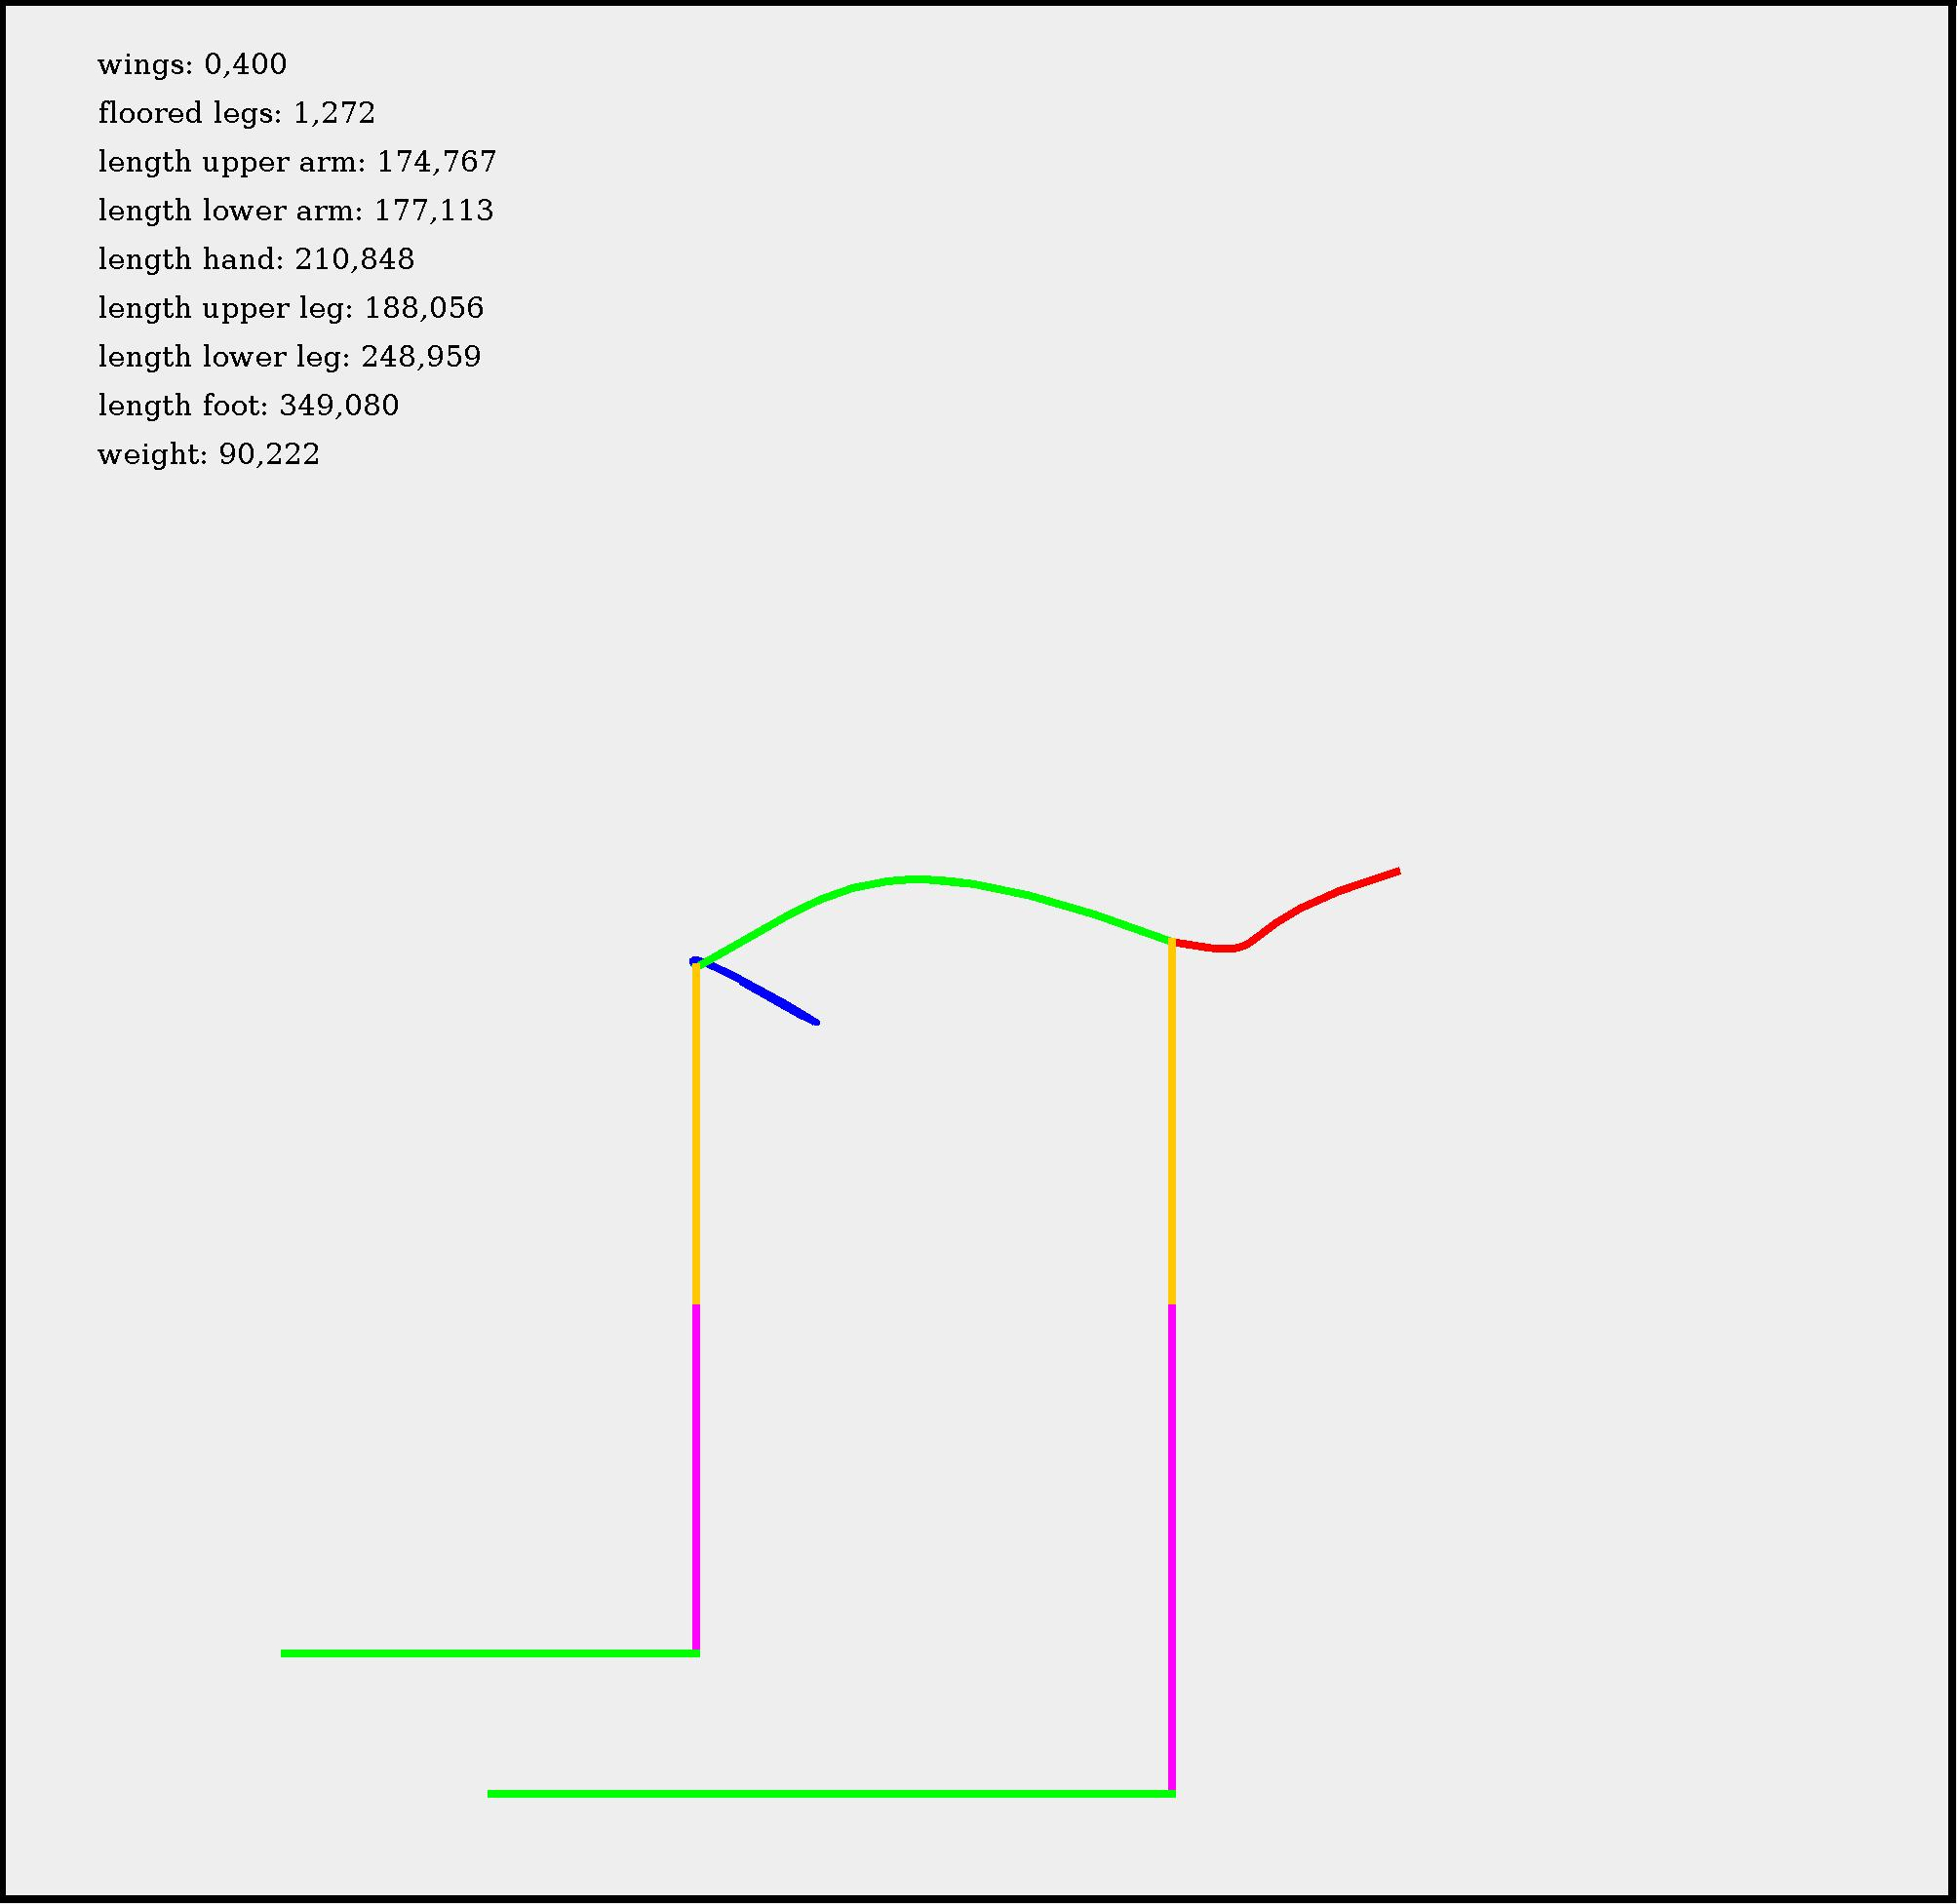
\includegraphics[width=0.4\textwidth]{../../PCA/animal_reconstructions_log_weight_downscaled_wings_legs_and_weight/6EV/Frosch_Ausschnitt.jpg}}~
  \subfloat[Eingabebild \cite{Spezielle_Zoologie}]{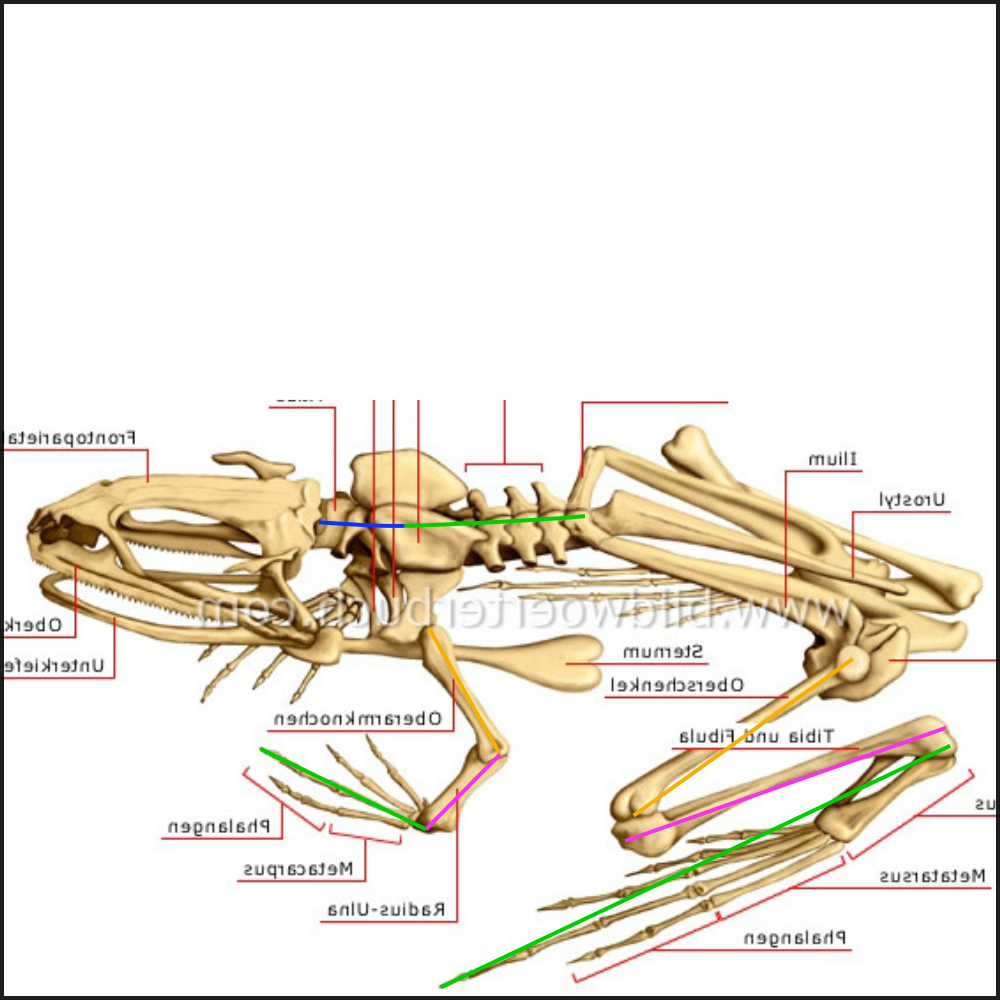
\includegraphics[width=0.4\textwidth]{../../PCA/Skelettbilder/Frosch_farbig.png}}
  
  \caption{Nicht visualisierte Daten der Rekonstruktion: \emph{Flügel} $0{,}4$, \emph{Beine mit Bodenkontakt} $1{,}27$, \emph{Gewicht} $90{,}2$kg; Originalwert für das \emph{Gewicht}: $0{,}01$kg.}
  \label{frosch}
 \end{figure}
\end{frame}

\begin{frame}
  \begin{figure}
   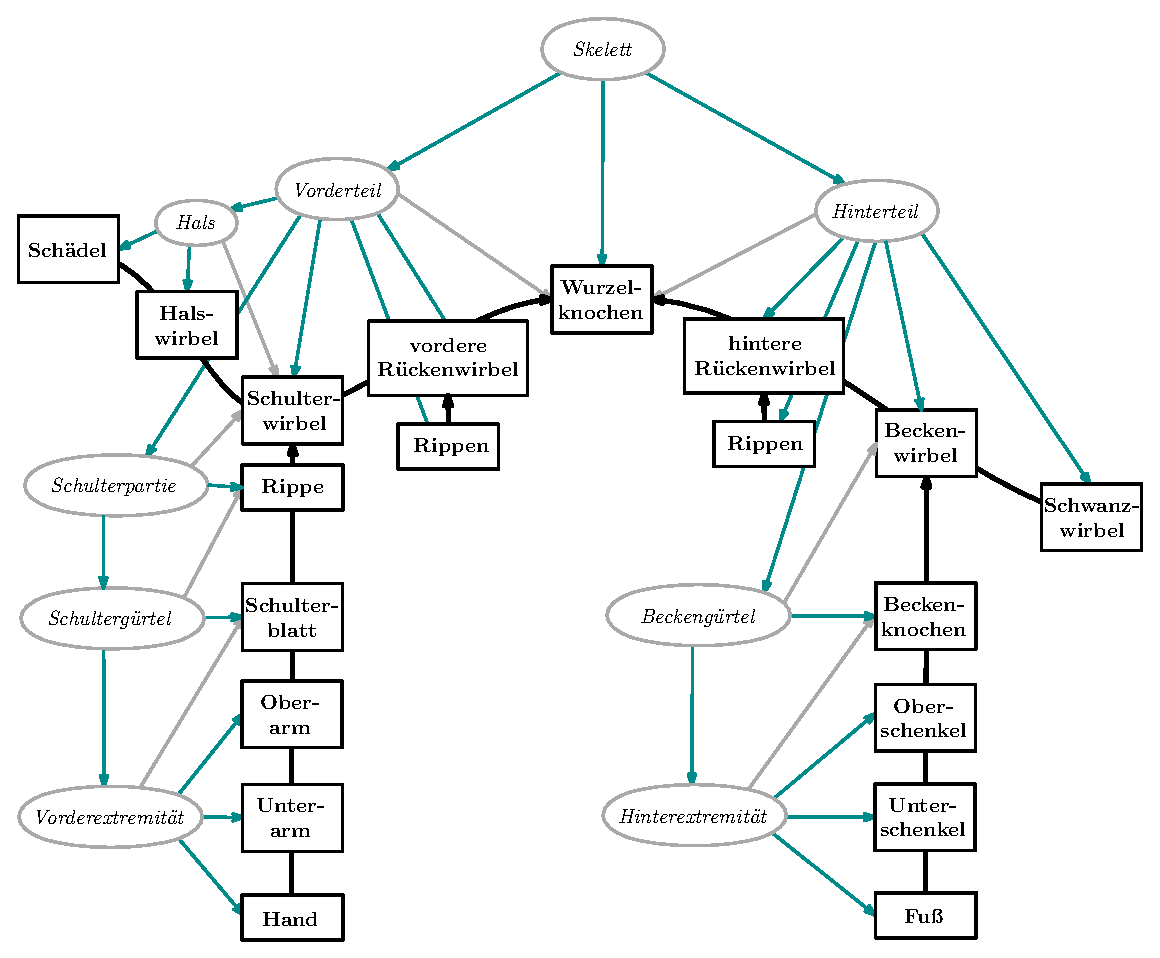
\includegraphics[height=0.9\textheight]{../graphics/grammarGraph_withoutLegend}
  \end{figure}
\end{frame}

\begin{frame}{Elefant: Vergleich mit dem Originalbild}
 \begin{figure}
  \subfloat{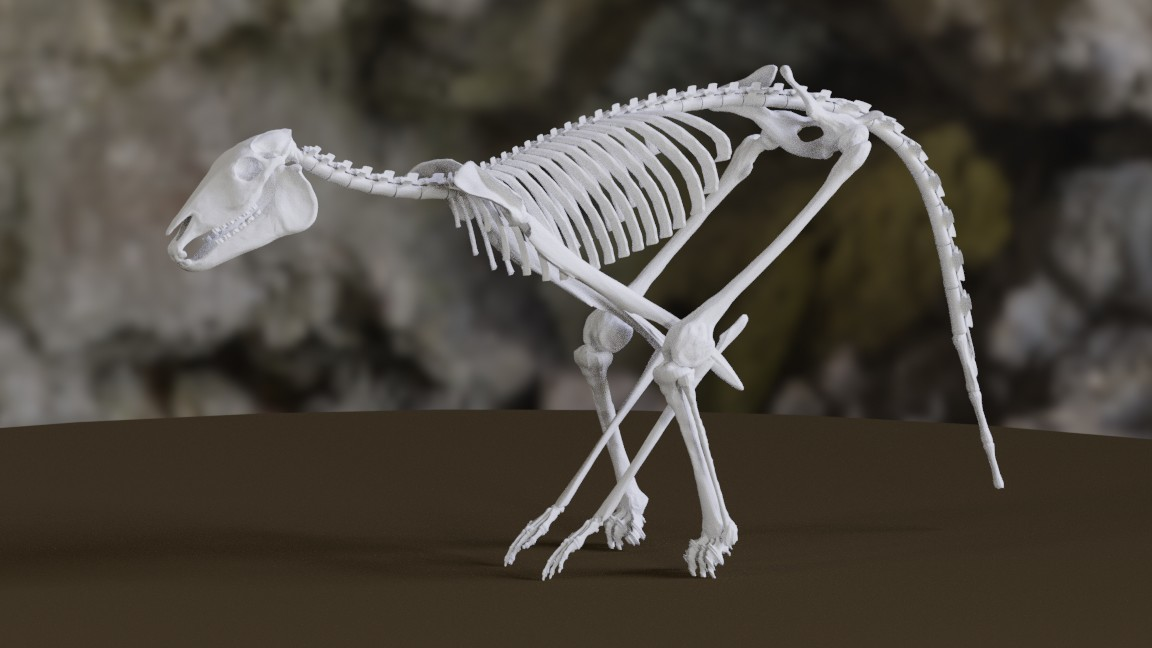
\includegraphics[width=0.5\textwidth]{../../java_skeleton_generation/example_skeletons/elefant.jpg}}~
  \subfloat{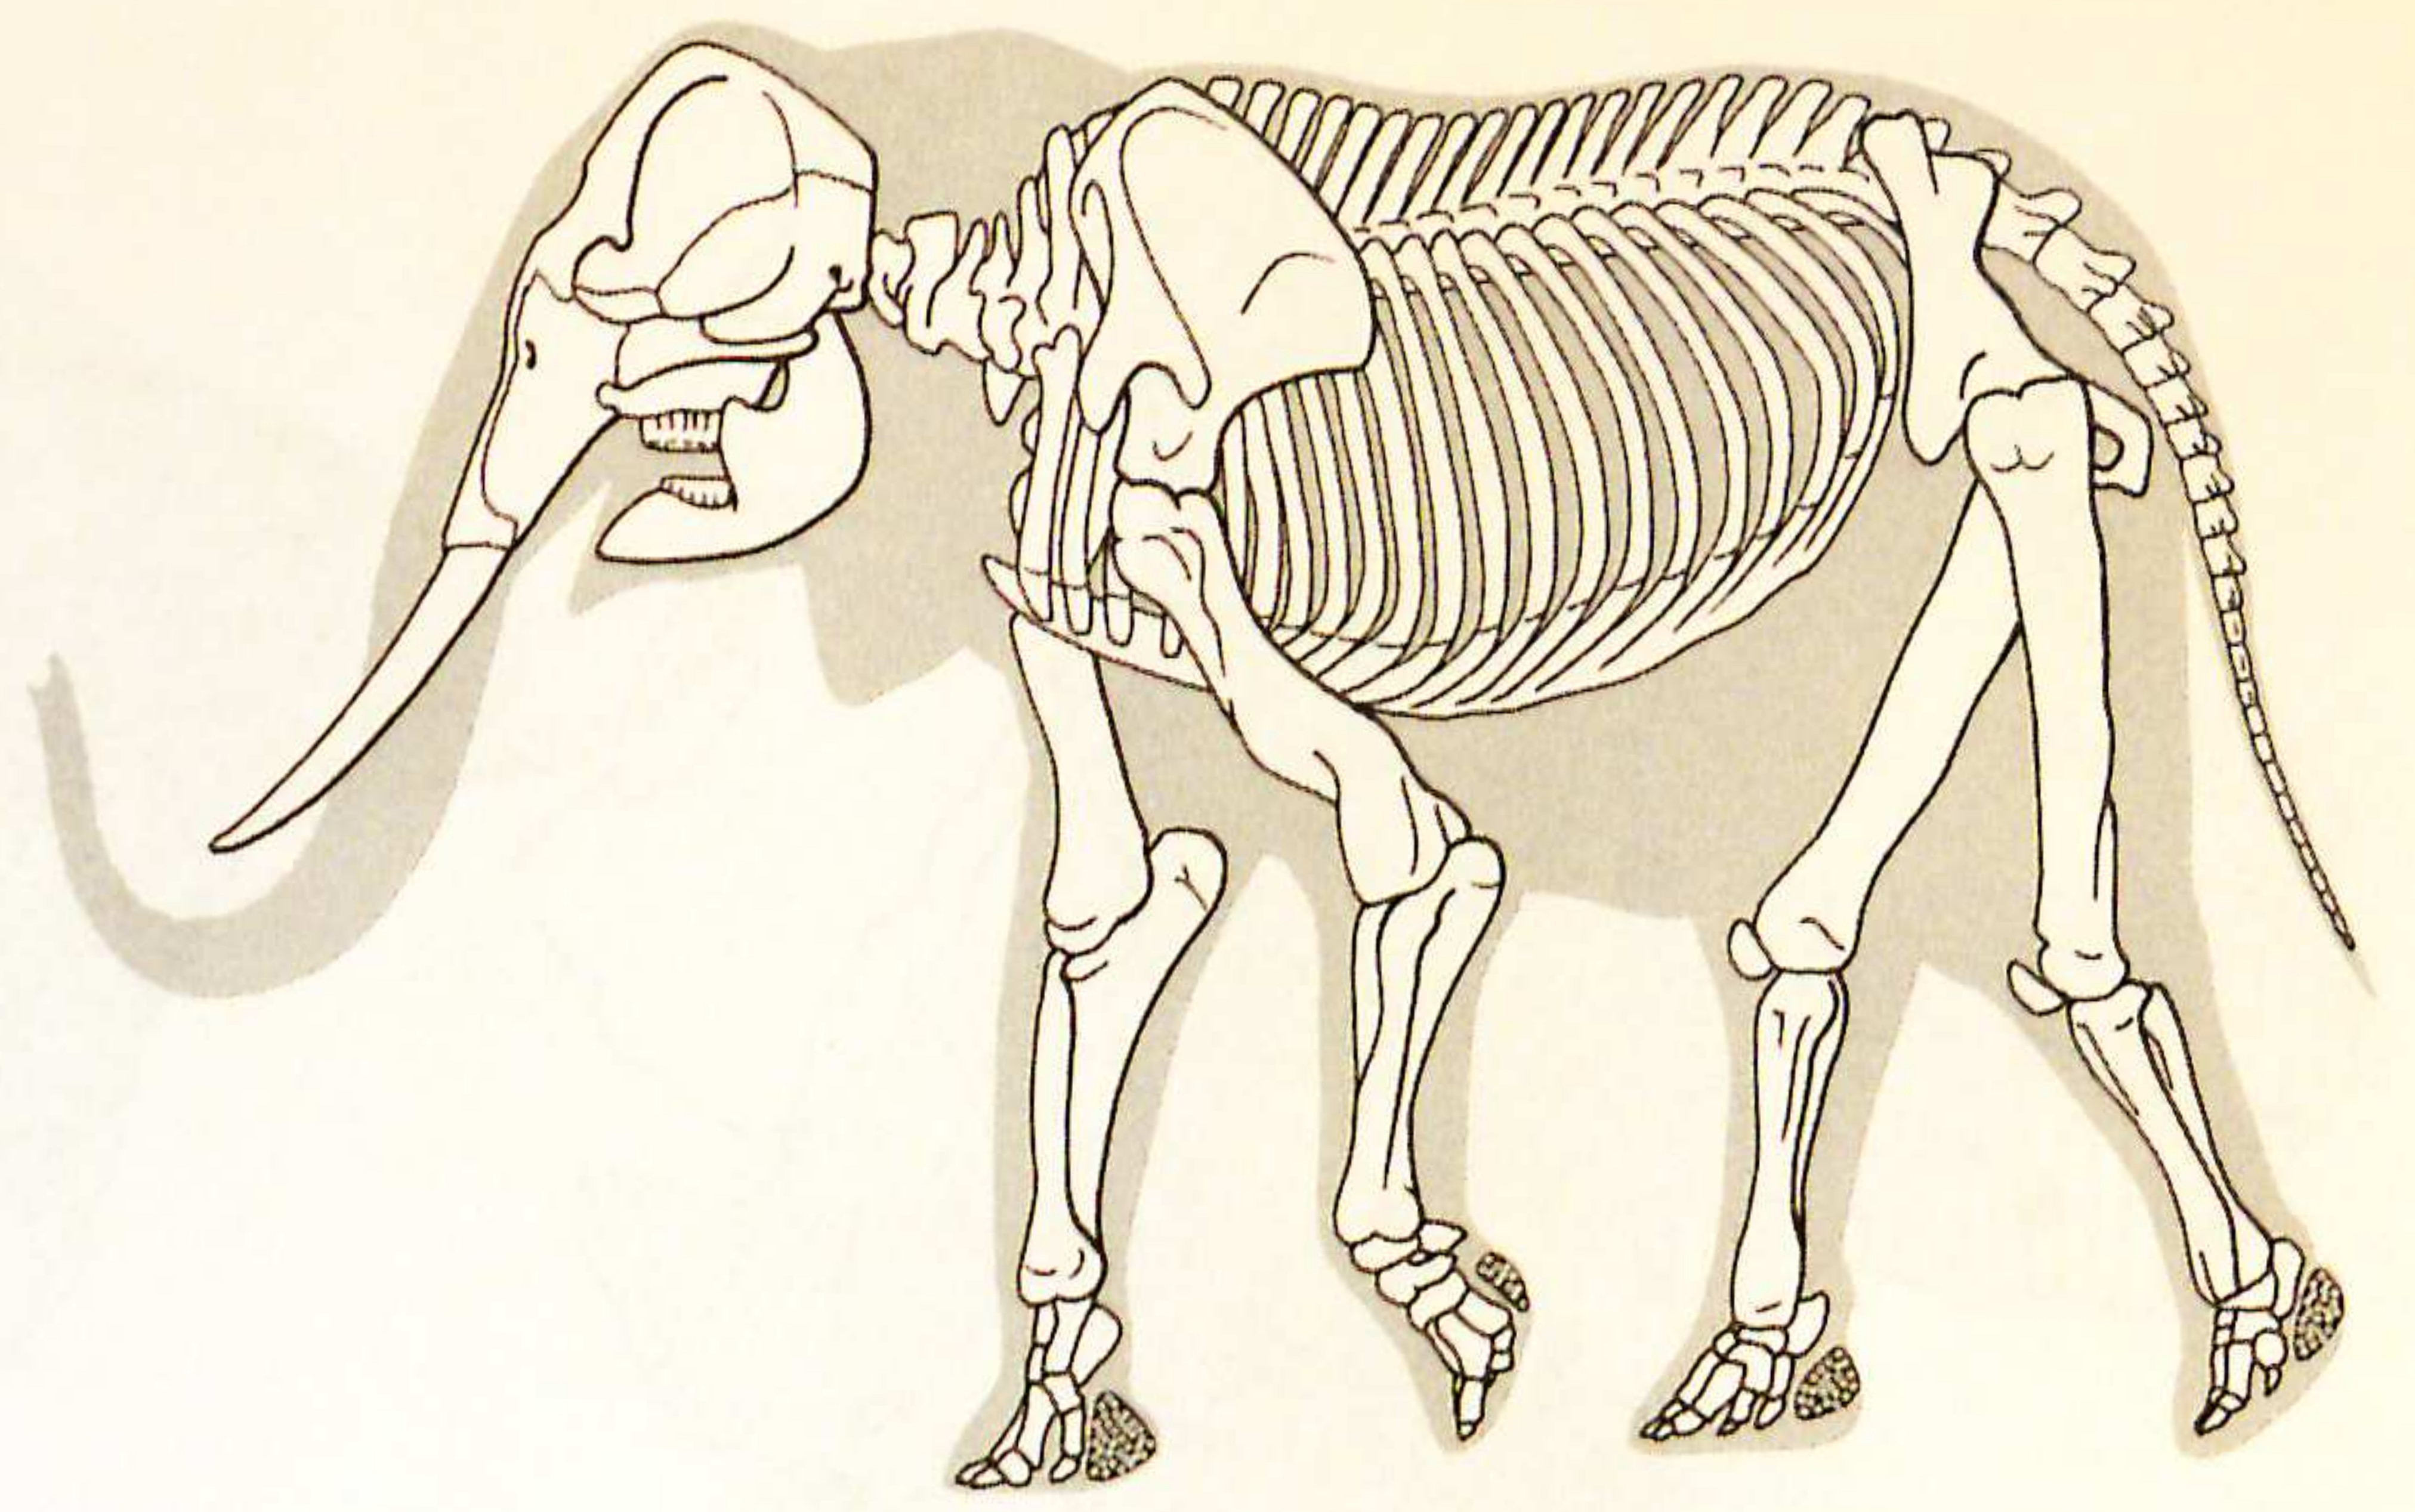
\includegraphics[width=0.5\textwidth]{../../PCA/Skelettbilder/Afrikanischer_Elefant.jpg}}
  \caption{\cite{Spezielle_Zoologie}}
 \end{figure}
\end{frame}

\end{document}
